\chapter{Evaluation}
\label{chapter:evaluation}

This chapter evaluates the proposed modeling and optimization framework of Chapter \ref{chapter:certifiable_trajectory_optimization}.
Section~\ref{sec:numerical_simulation_results} first validates the derived LGVIs for the
3D pendulum and the Acrobot through numerical simulations. Sections~\ref{sec:3d_pendulum_optimization_results}
and~\ref{sec:acrobot_optimization_results} then assess the corresponding sparse Moment-SOS
trajectory optimization problems. Finally, Section~\ref{subsec:acrobot_sdp_mpc_results}
examines the closed-loop performance of the SDP-MPC formulation for the Acrobot.

\section{Numerical Simulation Results} 
\label{sec:numerical_simulation_results}

In this section, numerical simulations are conducted to evaluate 
the correctness of the derived discrete integrators for mechanical models on 
Lie groups. In particular, the structure-preserving properties of the variational 
discretizations derived in Section~\ref{sec:properties_discrete_lagrangian_flow} are examined. 
The analysis focuses 
especially on the preservation of the momentum map associated with the symmetry 
of the system, the evolution on the Lie-group configuration manifold, and the 
long-time behaviour of the total energy. This validation is important since 
discrete mechanical models obtained by variational integration provide a reliable 
basis for certifiable trajectory optimization. If the discrete flow violates 
the manifold structure or introduces artificial drift in conserved quantities such 
as momentum, the resulting optimization model becomes less faithful to the 
underlying mechanics \cite{Lee2008}. Additionally, for the 3D-pendulum, the
numerical simulations are compared with classical fourth-order Runge-Kutta methods and projected Runge-Kutta methods 
on \(SO(3)\) as reference integrators \cite{CELLEDONI2003421, Hairer2000}.
(see Table~\ref{tab:integrator_comparison}).

\begin{table}[h]
\centering
\caption{Comparison of the considered integration methods properties.}
\label{tab:integrator_comparison}
\begin{tabular}{lcc}
\hline
\textbf{Method} & \textbf{Symplectic} & \textbf{Manifold Preserving} \\
\hline
Variational Integrator & \cmark & \cmark \\
RK4 & \xmark & \xmark \\
Projected RK4 & \xmark & \cmark \\
\hline
\end{tabular}
\end{table}

\paragraph{Runge--Kutta 4th order}
As a baseline integrator, the classical explicit fourth-order Runge-Kutta (RK4) method is applied to the continuous rigid-body equations written as a first-order system $(\dot{\bm{R}},\dot{\bm{\omega}}) = \bm{f}(\bm{R},\bm{\omega})$. For a system of the form
\begin{align}
    \dot{\bm{y}} = \bm{f}(\bm{y}),
\end{align}
the classical RK4 scheme computes the four stage values
\begin{subequations}\label{eq:rk4_stages}
\begin{align}
    (\bm{k}_1^{R}, \bm{k}_1^{\omega}) &= \bm{f}(\bm{R}_n, \bm{\omega}_n), \\
    (\bm{k}_2^{R}, \bm{k}_2^{\omega}) &= \bm{f}\!\left(\bm{R}_n+\frac{h}{2}\bm{k}_1^{R},\bm{\omega}_n+\frac{h}{2}\bm{k}_1^{\omega}\right), \\
    (\bm{k}_3^{R}, \bm{k}_3^{\omega}) &= \bm{f}\!\left(\bm{R}_n+\frac{h}{2}\bm{k}_2^{R},\bm{\omega}_n+\frac{h}{2}\bm{k}_2^{\omega}\right), \\
   (\bm{k}_4^{R}, \bm{k}_4^{\omega}) &= \bm{f}\!\left(\bm{R}_n+h\bm{k}_3^{R}, \bm{\omega}_n+h\bm{k}_3^{\omega}\right),
\end{align}
\end{subequations}
and updates the numerical solution according to
\begin{subequations}\label{eq:rk4_update}
\begin{align}
    \bm{R}_{n+1}
    &=
    \bm{R}_n
    +
    \frac{h}{6}
    \left(
    \bm{k}_1^{R} + 2\bm{k}_2^{R} + 2\bm{k}_3^{R} + \bm{k}_4^{R}
    \right), \\
    \bm{\omega}_{n+1}
    &=
    \bm{\omega}_n
    +
    \frac{h}{6}
    \left(
    \bm{k}_1^{\omega} + 2\bm{k}_2^{\omega} + 2\bm{k}_3^{\omega} + \bm{k}_4^{\omega}
    \right),
\end{align}
\end{subequations}
for each discrete-time step $n$ \cite{butcher2016numerical}.

The explicit RK4 method does not preserve the orthogonality constraint \(\bm{R}^\top \bm{R}=\bm{I}\) and leaves the configuration manifold $SO(3)$, since the rotation matrix $\bm{R}_n$ is updated additively in the vector space of $\mathbb{R}^{3 \times 3}$ \cite{CELLEDONI2003421}.

\paragraph{RK4 projected to $SO(3)$}

The explicit RK4 method is combined with a projection of the updated discrete-time rotation matrix $\bm{R}_n$ onto $SO(3)$ to satisfy the orthogonality constraint
\[
SO(3)
=
\left\{
\bm{R}\in\mathbb{R}^{3\times 3}
\;\middle|\;
\bm{R}^\top \bm{R}=\bm{I}_3,\ 
\det(\bm{R})=1
\right\}.\]
After performing the RK4 step in $\mathbb{R}^{3 \times 3}$, the singular value decomposition of the obtained rotation matrix \(\widetilde{\bm{R}}_{n+1}\) is computed as
\begin{align}
    \widetilde{\bm{R}}_{n+1}=\bm{U}\bm{\Sigma}\bm{V}^{\top},
\end{align}
followed by a reconstruction of the updated rotation matrix
\begin{align}
    \bm{R}_{n+1}=\bm{U}\bm{V}^{\top},
\end{align}
which is projected onto $SO(3)$ \cite{YanaiTakeuchiTakane2011SVD}. Consequently, $\bm{R}_{n+1}$ satisfies the orthogonality constraint, while the angular velocity $\bm{\omega}_{n+1}$ remains unchanged in the vector space $\mathbb{R}^{3}$. However, this method does not inherit structure-preserving properties of the Lie group variational integrator, for example, symplecticity or momentum conservation \cite{CELLEDONI2003421}. 

\subsection{3D Pendulum}
\label{subsec:3d_pendulum_numercial_simulation}

For evaluating the preservation of the geometric properties of the previously 
defined 3D-pendulum (see Section \ref{sec:discrete_3D_pendulum}), 
numerical simulations are conducted for the unforced and controlled cases. The rigid body is modeled as a uniform solid cylinder of length $l=\SI{1}{\meter}$ and radius $r=\SI{5}{\cm}$, with its center of mass at $\frac{l}{2}$. Thereby, the physical parameters characterizing the configuration manifold are chosen as 
\begin{align}
    m &= \SI{1}{\kilogram}, &
    g &= \SI{9.81}{\meter\per\second\squared}, \\
    \bm{\rho}_c &=
    \begin{bmatrix}
        0 & 0 & 0.5
    \end{bmatrix}^\top \si{\meter}, &
    \bm{e}_3 &=
    \begin{bmatrix}
        0 & 0 & 1
    \end{bmatrix}^\top.
\end{align}
 The inertia matrix about the center of mass can be taken from the inertia table given in \cite{RITInertiaTable216}. The rotations about the $x$- and $y$-axes are about the central diameters, with $J_{11,com}=J_{22,com}= \frac{1}{12}m(3r^2 + l^2)$, while the rotation about the gravity-direction $z$-axis has $J_{33,com}=\frac{1}{2} mr^2$. The off-diagonal terms are equal to zero, because the body-fixed frame is aligned with the principal axes of the cylindrically symmetric body \cite{Lee2008}. Additionally, the inertia matrix about the pivot in body-frame is obtained by the parallel axis theorem of \cite{Benacquista2018ClassicalMechanics} given by
\begin{align}
    \bm{J}
    =
    \bm{J}_{\mathrm{com}}
    +
    m\left(
        \|\bm{\rho}_c\|^2\bm{I}
        -
        \bm{\rho}_c\bm{\rho}_c^{\top}
    \right).
\end{align}
After substituting the chosen values, the 3D-pendulum's inertia matrix is given by
\begin{align}
    \bm{J}
    &=
    \begin{bmatrix}
        0.33396 & 0 & 0 \\
        0 & 0.33396 & 0 \\
        0 & 0 & 0.00125
    \end{bmatrix}
    \si{\kilogram\meter\squared}.
\end{align}
Given \eqref{eq:non-standard_inertia}, the non-standard inertia matrix is calculated as
\begin{align}
    \bm{J}_d
    &=
    \begin{bmatrix}
        0.000625 & 0 & 0 \\
        0 & 0.000625 & 0 \\
        0 & 0 & 0.333333
    \end{bmatrix}
    \si{\kilogram\meter\squared}.
\end{align}
Using the introduced computational approach of Section \ref{sec:discrete_computational_approach}, the derived discrete-time implicit Hamilton equations
of the unforced \eqref{eq:discrete_3D_pendulum_hamilton} and controlled \eqref{eq:forced_3D_pendulum_hamilton} 3D-pendulum are converted to an equivalent vector equation in $\mathbb{R}^3$ using the Cayley transformation. From \cite{ColomboJimenez2012SO3_Cayley}, the corresponding nonlinear vector equation $\bm{0} = \bm{A}(\bm{f})$ of the 3D-pendulum is taken as
\begin{equation}\label{eq:simulation_3D_pendulum_vector_equation}
    \bm{0} = \bm{a}+\bm{a} \times \bm{f} + \bm{f}(\bm{a}^\top \bm{f})-2 \bm{J} \bm{f} = \bm{A}(\bm{f}),
\end{equation}
with $\bm{a}= h (\bm{\Pi}_k + \frac{h}{2} \bm{\tau}_{g,k})$. Additionally, \cite{ColomboJimenez2012SO3_Cayley} defines its Jacobian $\nabla \bm{A}\!\left(\bm{f}\right)$ as
\begin{align}\label{eq:Caley_Jacobian}
\nabla \bm{A}(\bm{f})
=
\hat{\bm{a}}
+
(\bm{a}^{\top}\bm{f})\bm{I}
+
\bm{f}\bm{a}^{\top}
-
2\bm{J}.
\end{align}
The tolerance for the Newton iteration is defined by $\left\lVert \bm{f}^{(i+1)} - \bm{f}^{(i)} \right\rVert < 10^{-12}$. The initial conditions are taken from \cite{Lee2008} 
\begin{align}
\bm{f}^0 &= (2 \bm{J} - \hat{\bm{a}})^{-1}\bm{a},&
    \bm{R}_0 &= \bm{I}, &
    \bm{\omega}_0 &=
    \begin{bmatrix}
        4.14 & 4.14 & 4.14
    \end{bmatrix}^{\top}\si{\radian\per\second},
\end{align} where $\bm{f}^0$ is the linearized solution of
\eqref{eq:simulation_3D_pendulum_vector_equation}.
In the following, the numerical simulation is plotted against time $t_k = kh$. 
The corresponding implementation is documented in the GitHub repository \cite{Elshani2026CTO_GitHub}.

\subsubsection{Unforced 3D-Pendulum}

\begin{figure}[t]
    \centering
    \begin{minipage}{0.49\textwidth}
        \centering
        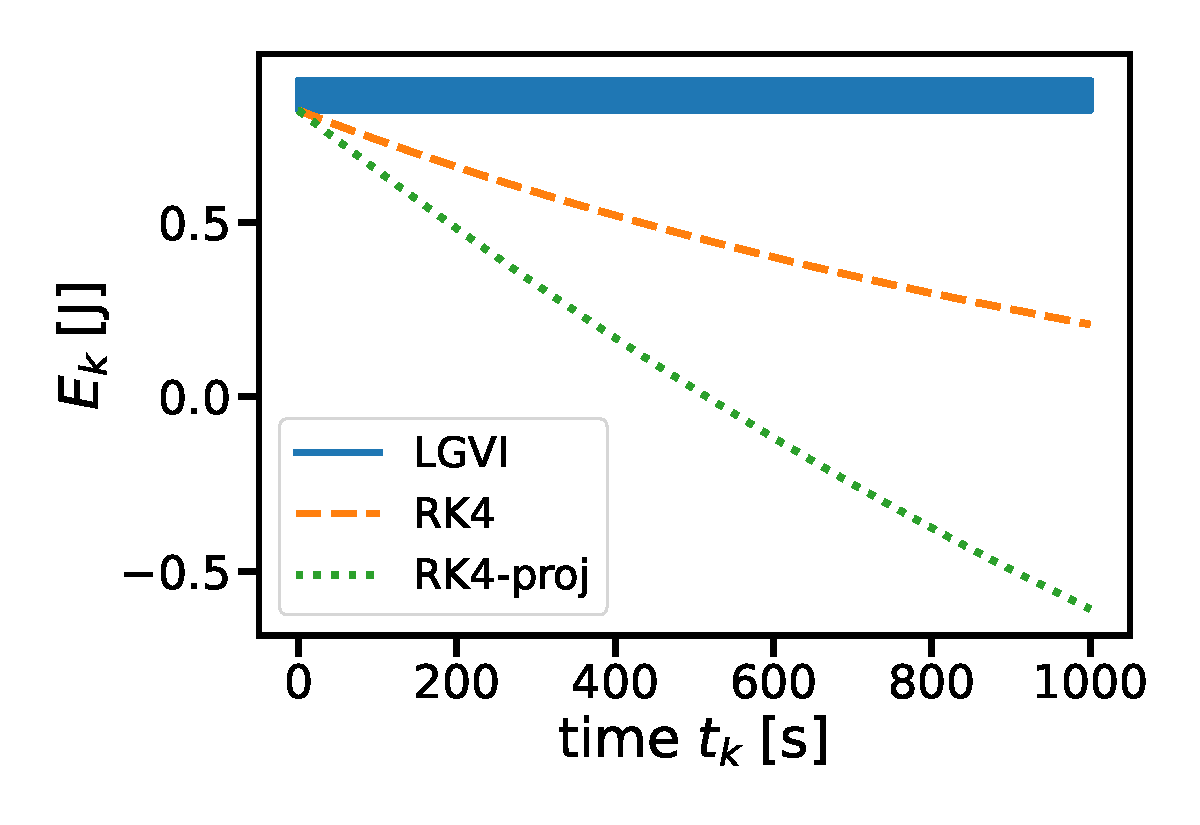
\includegraphics[width=\textwidth]{pics/Numerical_Simulation/Total_Energy.pdf}
        \caption*{(a) Total energy $E_k$.}
    \end{minipage}
    \hfill
    \begin{minipage}{0.49\textwidth}
        \centering
        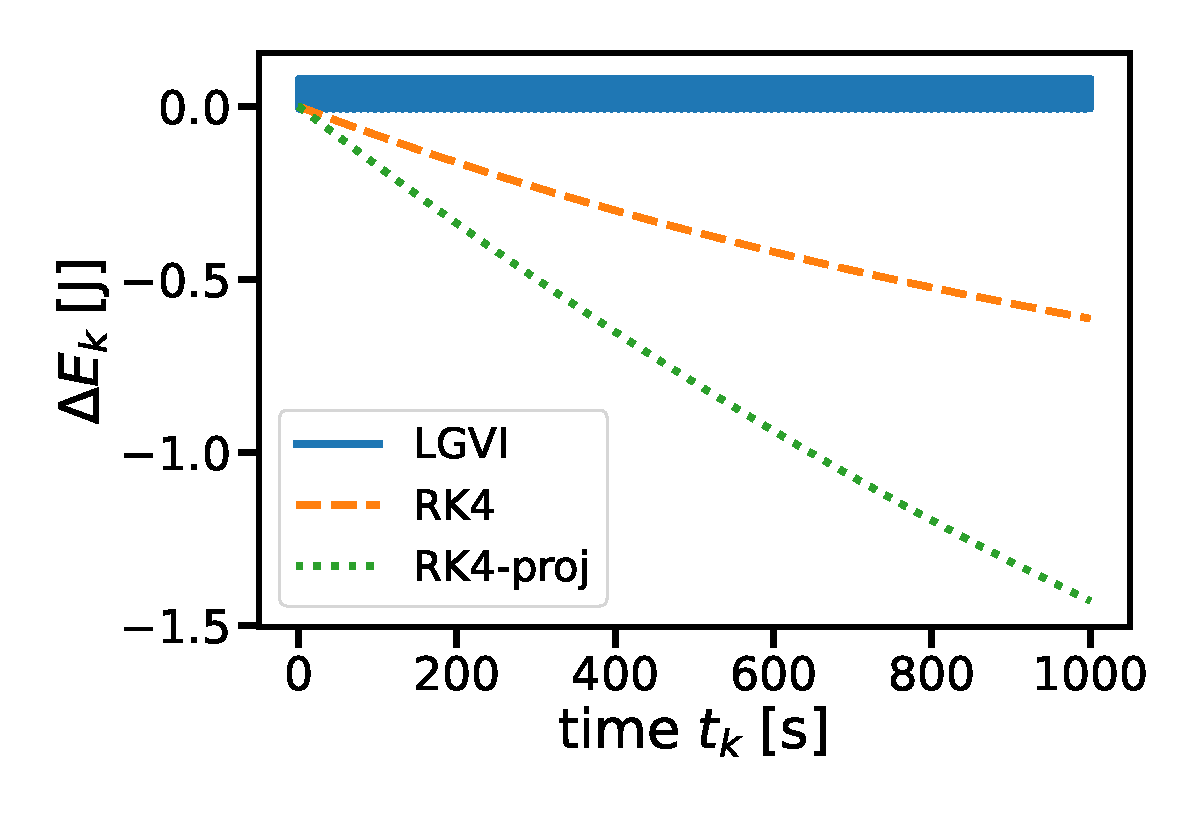
\includegraphics[width=\textwidth]{pics/Numerical_Simulation/Delta_E.pdf}
        \caption*{(b) Energy deviation $\Delta E_k$.}
    \end{minipage}

    \vspace{0.5em}

    \begin{minipage}{0.49\textwidth}
        \centering
        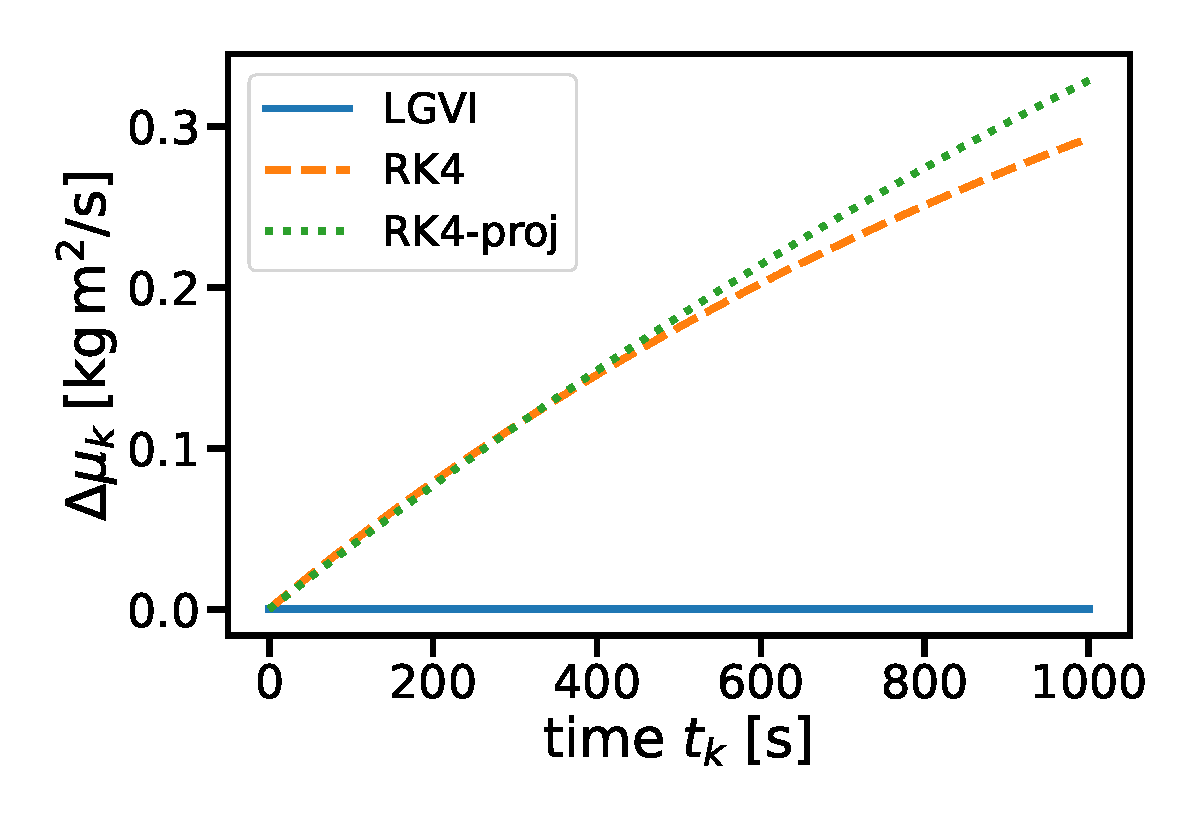
\includegraphics[width=\textwidth]{pics/Numerical_Simulation/Momentum_error.pdf}
        \caption*{(c) Momentum error $\Delta \mu_k$.}
    \end{minipage}
    \hfill
    \begin{minipage}{0.49\textwidth}
        \centering
        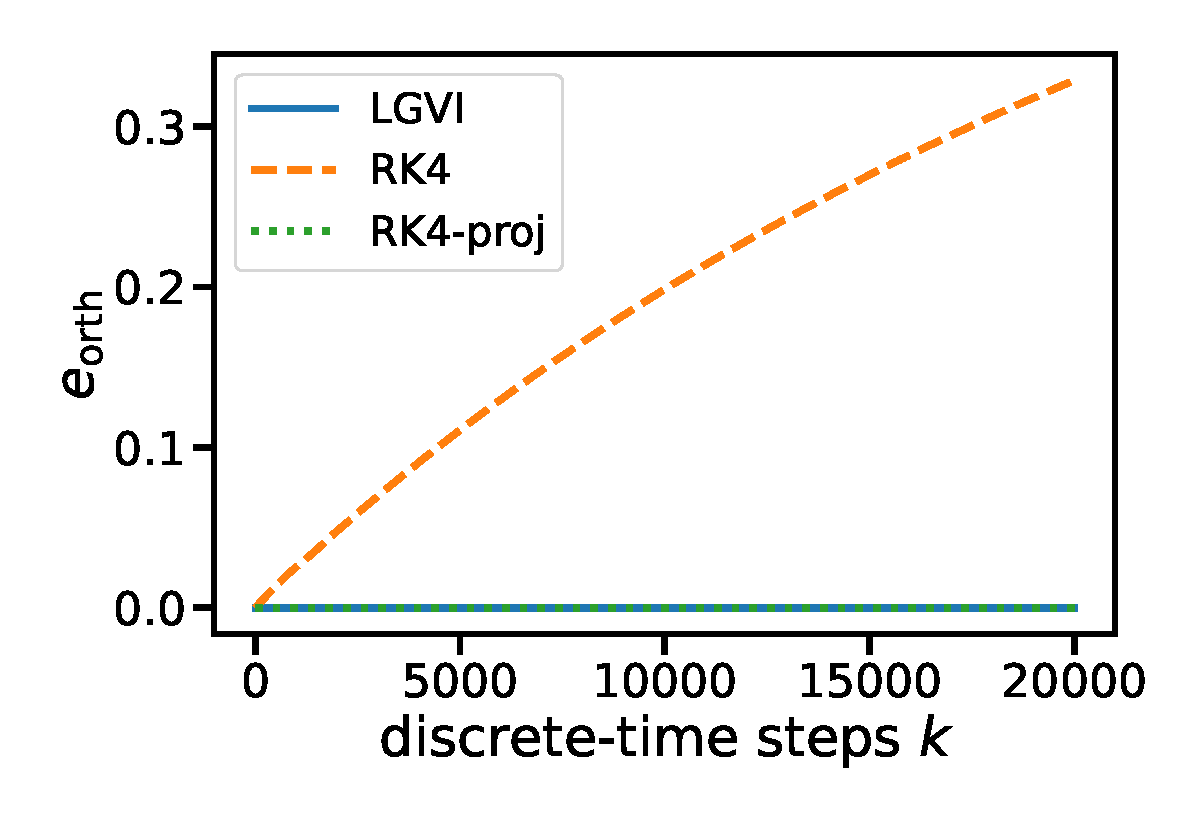
\includegraphics[width=\textwidth]{pics/Numerical_Simulation/Orthogonality_error.pdf}
        \caption*{(d) Orthogonality error $e_{orth}$.}
    \end{minipage}

    \caption{Comparison of the numerical preservation properties for the unforced $3$D pendulum.}
    \label{fig:simulation_results_3d_pendulum}
\end{figure}

The results of the numerical simulation for the unforced case, with 
$\bm{u}_k=\bm{0}$, are shown in Fig.~\ref{fig:simulation_results_3d_pendulum}. 
The simulation is performed over $20000$ discrete-time steps with a step size of 
$h=\SI{0.05}{\second}$. Thereby, the accuracy of the different integrator methods given in Table \ref{tab:integrator_comparison} is compared by plotting the corresponding total energy
\[
 E_k
    =
    \frac{1}{2}\bm{\omega}_k^{\top}\bm{J}\bm{\omega}_k
    -
    mg\,\bm{e}_3^{\top}\bm{R}_k\bm{\rho}_c,
\]
and its deviation $\Delta E_k = E_k - E_0$, the angular momentum error along the gravity direction
\[
\Delta \mu_k= \bm{e}_3^{\top}\bm{R}_k\bm{\Pi}_k - \bm{e}_3^{\top}\bm{R}_0\bm{\Pi}_0,
\]
defined in \cite{Lee2008}, and the orthogonality error 
\[
e_{\mathrm{orth},k} = \left\|\bm{I}-\bm{R}_k^{\top}\bm{R}_k\right\|_F.
\]

The total energy (see Fig. \ref{fig:simulation_results_3d_pendulum} (a)) and the corresponding energy deviation (see Fig. \ref{fig:simulation_results_3d_pendulum} (b)) illustrate the energy-preserving behavior of the Lie Group Variational Integrator (LGVI) over a long-time discrete flow. The energy remains close to the reference level with only small bounded oscillations because the symplectic method exactly solves a perturbed Hamiltonian \cite{Hairer1994}. However, RK4 and projected RK4 display a clear drift of the energy away from its true value, which remains constant for this unforced model.

Moreover, the momentum error (see Fig. \ref{fig:simulation_results_3d_pendulum} (c)) confirms that the LGVI method preserves the momentum, as validated for continuous time in \ref{sec:continuous_3D_pendulum_momentum_validation}. The computational results for RK4 and its projection onto $SO(3)$ show that these methods drift from the initial momentum value because they do not preserve the total angular momentum \cite{Lee2008}. In particular, projected RK4 has a larger discrepancy because it enforces $\bm{R}^\top\bm{R} = \bm{I}$ while leaving the angular velocity $\bm{\omega}$ unchanged, which influences the momentum.

Lastly, the orthogonality error highlights that the LGVI preserves the structure of the Lie group configuration manifold, as depicted in Fig. \ref{fig:simulation_results_3d_pendulum} (d). A similar result is obtained for projected RK4, while classical explicit RK4 violates the orthogonality constraint. For RK4, $e_{orth}$ increases linearly with the number of simulation time steps.

Consequently, only the LGVI preserves the manifold structure together with the momentum and energy behaviour over a long-time horizon. Although RK4 can be projected onto the Lie group manifold $SO(3)$, it cannot preserve the momentum and exhibits long-term energy drift.

\subsubsection{Controlled 3D-Pendulum}

In the controlled case, the previously derived free dynamics of the 3D-pendulum
are extended by an external body-fixed control moment. Following the control
structure defined in \eqref{eq:external_control_moment_3D_pendulum}, the time-dependent control parameter is chosen as
\begin{align}
    \label{eq:controlled_3d_pendulum_input_parameter}
    \bm{u}_p(t)
    =
    \begin{bmatrix}
        0.15\sin(0.5t) \\
        0.10\cos(0.25t) \\
        0
    \end{bmatrix}.
\end{align}
The corresponding discrete control input is obtained by evaluating the control law
at the discrete time nodes $\bm{u}_{p,k} =\bm{u}_p(t_k)$. Thus, the control input acts as a body-fixed external moment that is orthogonal to
the gravity direction expressed in the body frame, given by
$\bm{R}_k^{\top}\bm{e}_3$. Consequently, the control moment has no component
along this direction.

For the RK4 simulation, the continuous-time Hamilton equations \eqref{eq:continuous_3D_pendulum_hamilton} are used, 
with the control input $\bm{u}(t)$ added according to the Lagrange--d'Alembert principle of Section \ref{sec:discrete_forced_lagrangian}.
With the body angular momentum defined by $\bm{\Pi} = \bm{J}\bm{\omega}$,
the forced continuous-time equations of motion are written as
\begin{subequations}
\label{eq:controlled_3d_pendulum_continuous_RK4}
\begin{align}
    \dot{\bm{\Pi}}
    &=
    mg\,\bm{\rho}_c
    \times
    \bm{R}^{\top}\bm{e}_3
    -
    \bm{J}^{-1}\bm{\Pi}
    \times
    \bm{\Pi}
    +
    \bm{u}(t),
    \label{eq:controlled_3d_pendulum_continuous_momentum}
    \\
    \dot{\bm{R}}
    &=
    \bm{R}
    \left(
        \bm{J}^{-1}\bm{\Pi}
    \right)^{\wedge}.
    \label{eq:controlled_3d_pendulum_continuous_kinematics}
\end{align}
\end{subequations}
In contrast to the unforced case, the external input acts on the system.
Therefore, the total energy and the momentum map are no longer expected to be
conserved.

For the Lie group variational integrator, the forced discrete Hamilton equations
derived in \eqref{eq:forced_3D_pendulum_hamilton} are applied. The implicit
equation for the relative update $\bm{F}_k$ is again solved by using the Cayley
transformation. Compared to the unforced case, only the vector
$\bm{a}$ in \eqref{eq:simulation_3D_pendulum_vector_equation} changes due to
the additional control input. For the controlled dynamics, it is given by
\begin{align}
    \label{eq:controlled_3d_pendulum_cayley_a}
    \bm{a}
    =
    h
    \left(
        \bm{\Pi}_k
        +
        \frac{h}{2}
        \left(
            \bm{\tau}_{g,k}+\bm{u}_k
        \right)
    \right).
\end{align}
Therefore, the nonlinear vector equation \eqref{eq:simulation_3D_pendulum_vector_equation}
and its Jacobian \eqref{eq:Caley_Jacobian} are solved equivalently to the unforced simulation, with
the modified vector $\bm{a}$ including the control contribution. After computing
$\bm{f}_k$, the relative attitude update is obtained from the Cayley transformation
and the discrete-time states are propagated according to the forced LGVI. The corresponding implementation
is documented in the GitHub repository \cite{Elshani2026CTO_GitHub}.

The numerical simulation of the controlled 3D-pendulum compares the classical RK4 method with the forced
LGVI. Since the purpose of this experiment is to evaluate the behaviour of the
forced variational discretization under an external input, the projected RK4 method
is not considered in this comparison. The same physical parameters and initial
conditions as in the unforced case are used.

Fig.~\ref{fig:forced_3d_pendulum_results} shows the numerical results for the
controlled 3D-pendulum. The simulation is performed over $N=100000$ discrete-time
steps with step size $h=\SI{0.001}{\second}$. This shorter time interval is chosen
because the differences between the RK4 method and the forced LGVI already become
visible after a small number of time steps. During approximately the first eight
seconds, both methods show almost identical behaviour, which indicates that the
derived forced equations and their implementation are consistent. As the simulation
progresses, however, the trajectories begin to separate.

\begin{figure}[t]
    \centering
    \begin{minipage}{0.49\textwidth}
        \centering
        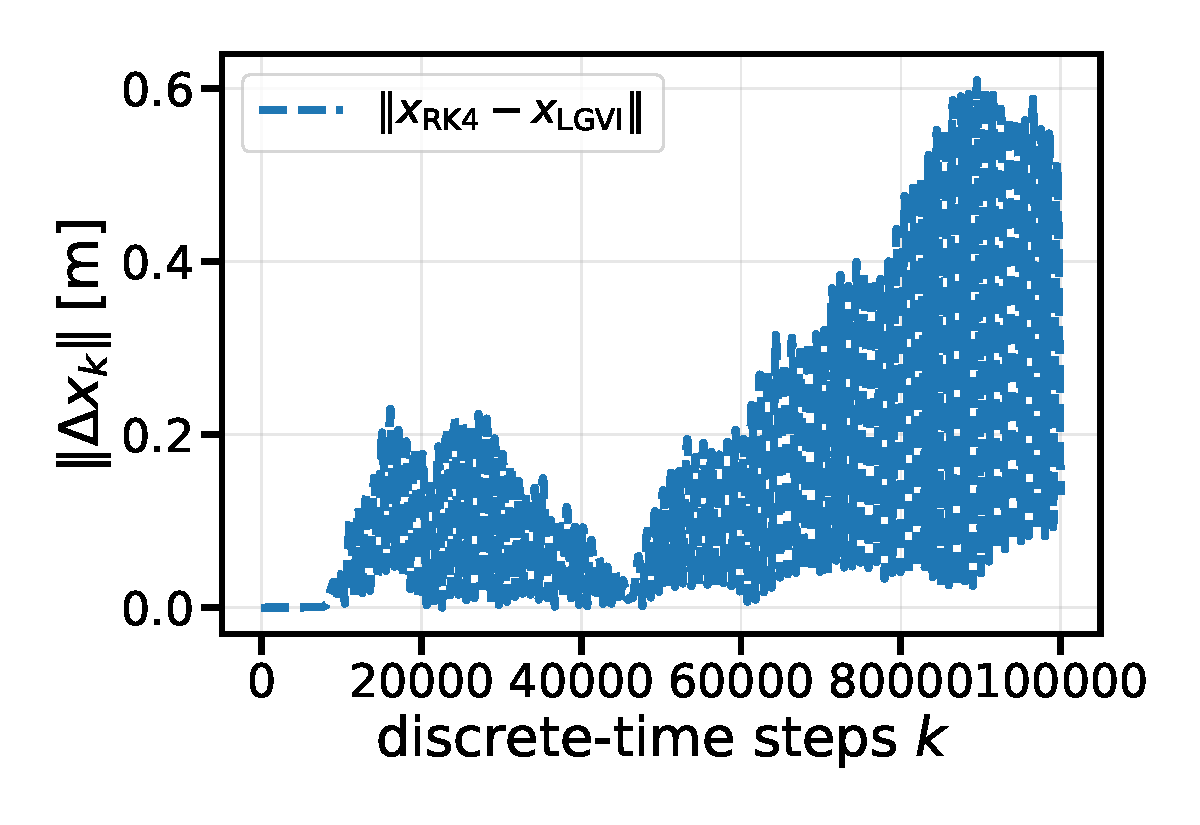
\includegraphics[width=\textwidth]{pics/Numerical_Simulation/Forced_3D_Pendulum_Trajectory.pdf}
        \caption*{(a) Position error norm $\|\Delta \bm{x}_k \||$.}
    \end{minipage}
    \hfill
    \begin{minipage}{0.49\textwidth}
        \centering
        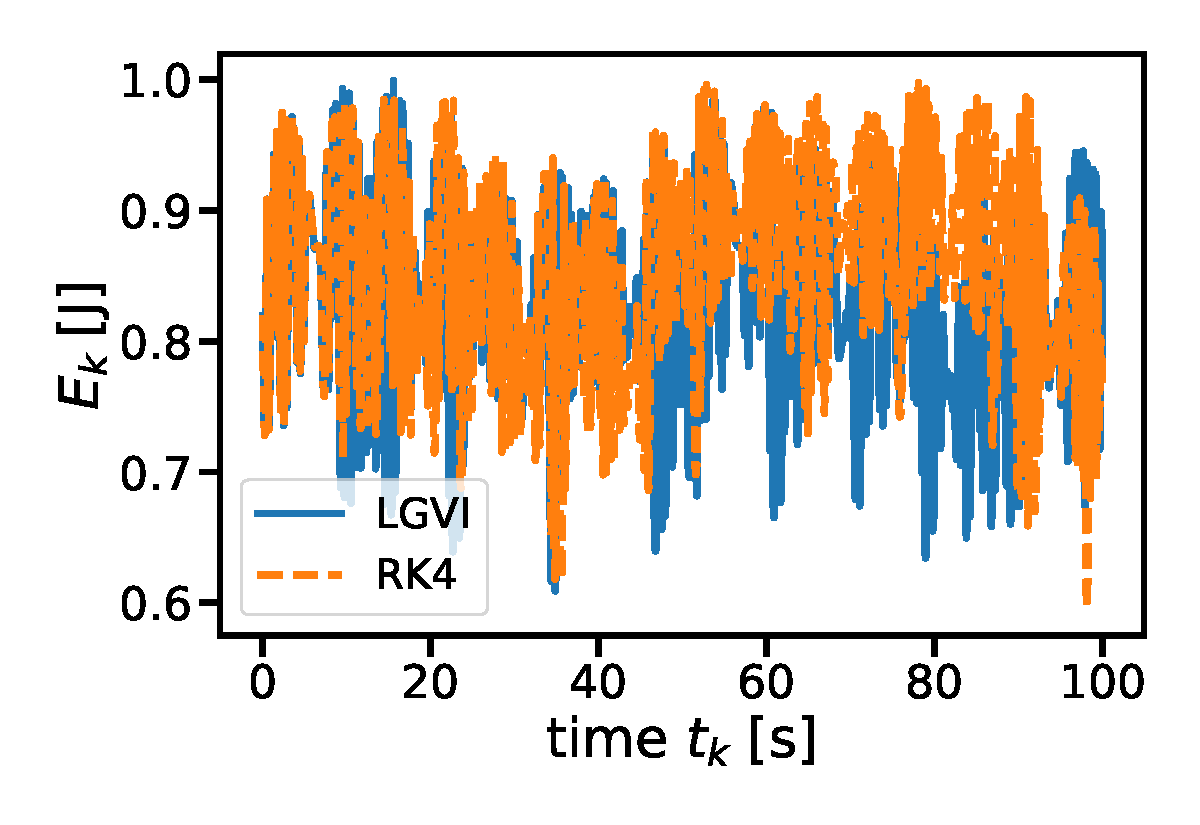
\includegraphics[width=\textwidth]{pics/Numerical_Simulation/Forced_3D_Pendulum_Ek.pdf}
        \caption*{(b) Total energy $E_k$.}
    \end{minipage}

    \vspace{0.5em}

    \begin{minipage}{0.49\textwidth}
        \centering
        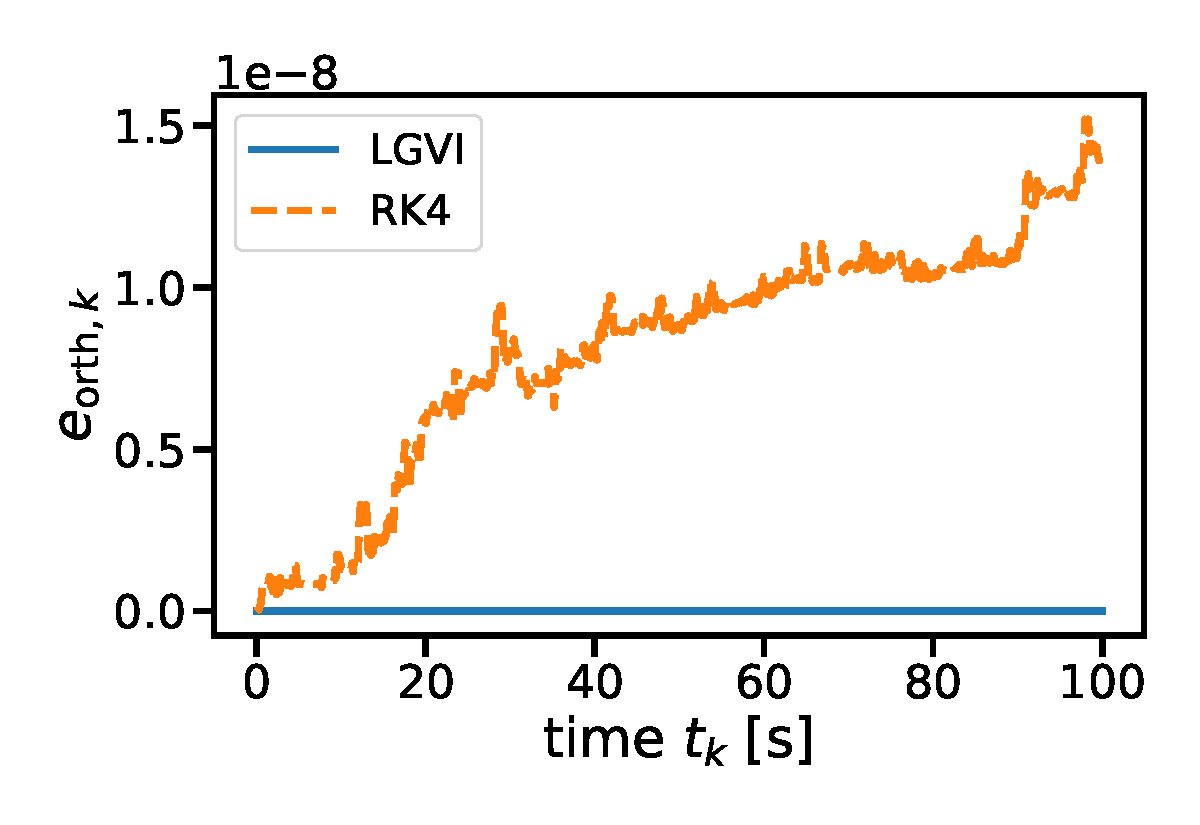
\includegraphics[width=\textwidth]{pics/Numerical_Simulation/Forced_3D_Pendulum_Orth_Error.pdf}
        \caption*{(c) Orthogonality error $e_{\mathrm{orth},k}$.}
    \end{minipage}
    \hfill
    \begin{minipage}{0.49\textwidth}
        \centering
        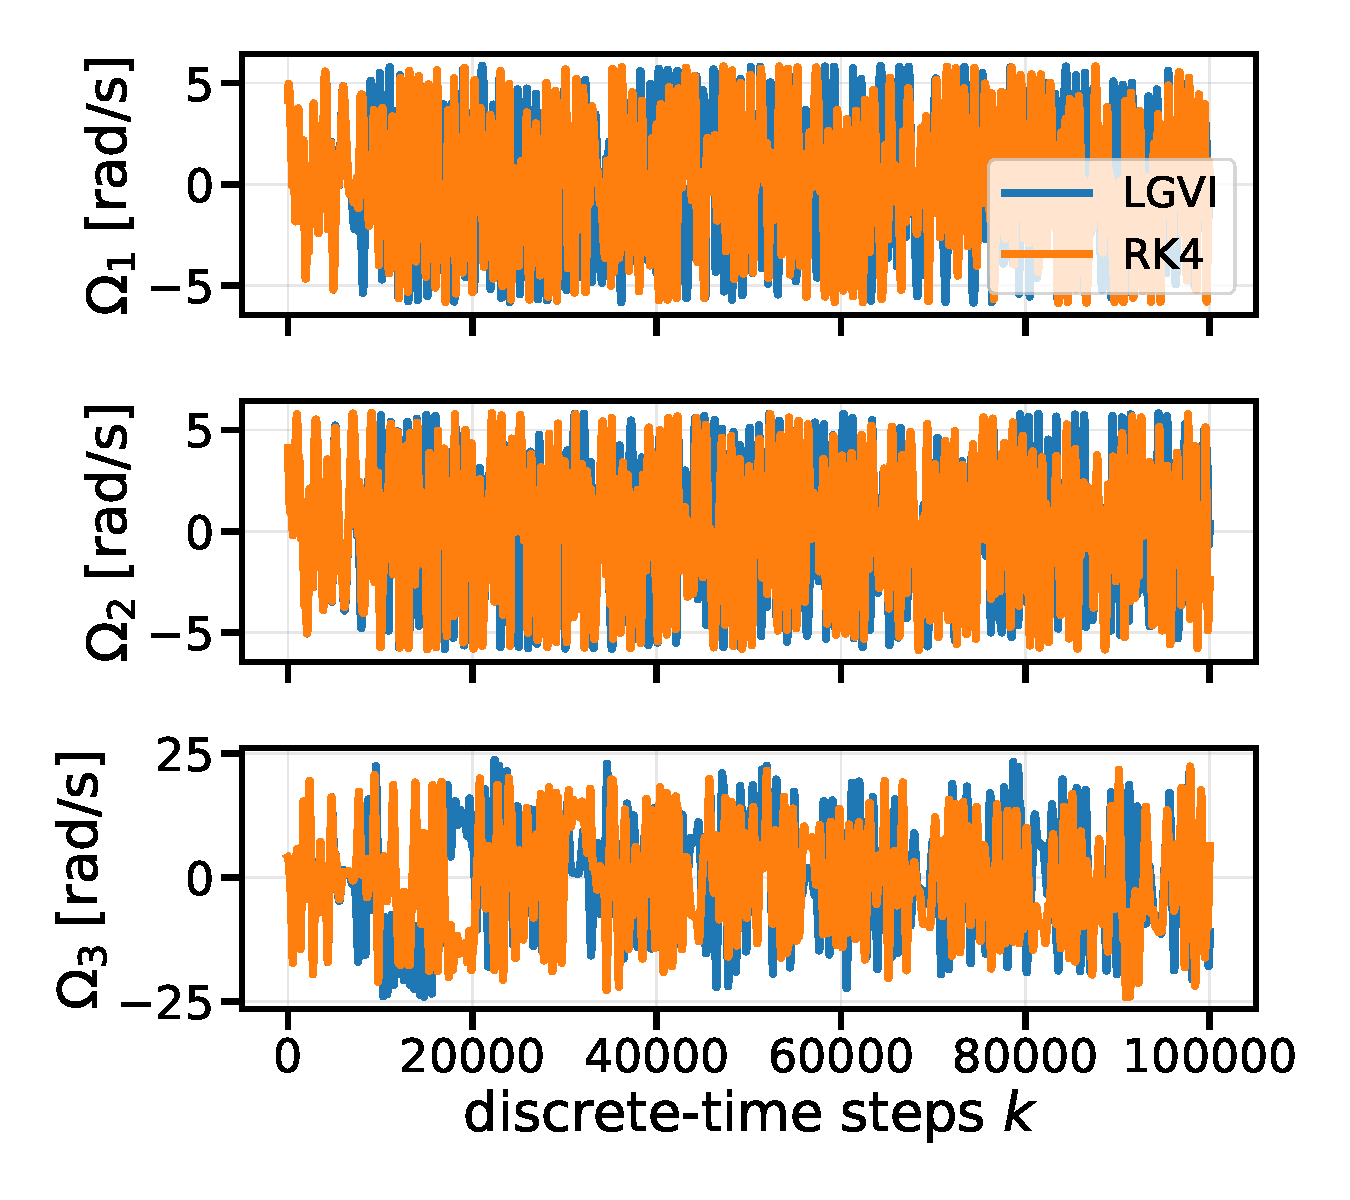
\includegraphics[width=\textwidth]{pics/Numerical_Simulation/Forced_3D_Pendulum_Omega.pdf}
        \caption*{(d) Angular velocity components $\bm{\omega}_k$.}
    \end{minipage}

    \caption{Comparison of the forced LGVI and RK4 simulation for the controlled $3$D pendulum.}
    \label{fig:forced_3d_pendulum_results}
\end{figure}

The position error in Fig.~\ref{fig:forced_3d_pendulum_results}~(a) is computed
from the center-of-mass position $\bm{x}_k=\bm{R}_k\bm{\rho}_c$,
as
\begin{align}
    \left\|\Delta \bm{x}_k\right\|_2
    =
    \left\|
        \bm{x}_{k,\mathrm{RK4}}
        -
        \bm{x}_{k,\mathrm{LGVI}}
    \right\|_2 .
\end{align}
The plot shows that the position error $\Delta \bm{x}_k$ is initially close to zero, but increases
over the simulation. Therefore, both methods reproduce the same short-time motion,
while their trajectories separate after a certain number of time steps. This behaviour is
expected for forced rigid-body dynamics, where small numerical
differences in the attitude $\bm{R}_k$ and momentum update $\bm{\Pi}_k$ can accumulate over time.

The total energy is shown in Fig.~\ref{fig:forced_3d_pendulum_results}~(b).
In contrast to the unforced case, the total mechanical energy is not expected to be
conserved, since the external input $\bm{u}_{p,k}$ acts on the system. It is observed that
the energetic behaviour of LGVI and RK4 under the same applied control
input follows a similar trend at the beginning, but small deviations
appear as the trajectories begin to separate, which is consistent with the position error.

The orthogonality error $e_{\mathrm{orth},k}$ is illustrated in Fig.~\ref{fig:forced_3d_pendulum_results}~(c).
Again, the plot confirms that the LGVI preserves the Lie group structure by staying on the manifold and updating the attitude through
$\bm{R}_{k+1}=\bm{R}_k\bm{F}_k$ with $\bm{F}_k\in SO(3)$. For RK4, the attitude is
updated additively in the surrounding vector space using the discrete update map \eqref{eq:rk4_update}. Over the short interval and due
to the small step size $h$, the orthogonality error remains small, but it is not preserved and increases over time.

Finally, Fig.~\ref{fig:forced_3d_pendulum_results}~(d) compares the angular
velocity components $\bm{\omega}_k$. In the discrete Hamiltonian formulation, the angular velocity
is recovered from the body angular momentum by
\begin{align}
    \hat{\bm{\omega}}_k
    =
    (\bm{J}^{-1}\bm{\Pi}_k)^\wedge,
\end{align}
discretizing and solving \eqref{eq:continuous_3D_pendulum_momentum} for $\hat{\bm{\omega}}_k$.
The angular velocity components of LGVI and RK4 are equal at the beginning of the
simulation, but begin to differ after a small number of steps. This confirms the
same behaviour observed in the position error $\Delta \bm{x}_k$ and the plotted energy $E_k$.
The 3D-Pendulum numerical simulation using external control inputs produces
consistent short-time dynamics of LGVI and RK4, while the numerical trajectories produced by the two methods separate as the
simulation continues.

\subsection{Acrobot}
\label{subsec:evaluation_acrobot}

To evaluate the preservation of the geometric properties of the previously defined Acrobot (see Section \ref{subsection:discrete_Acrobot}), 
numerical simulations are conducted for the unforced and controlled cases similar to those conducted for the 3D-pendulum 
in Section \ref{subsec:3d_pendulum_numercial_simulation}. 
In contrast to the 3D-pendulum, the Acrobot is a constrained multi-body system in maximal coordinates with the configuration 
\[
q_k =
\left(
\bm{x}_{1,k},
\bm{R}_{1,k},
\bm{x}_{2,k},
\bm{R}_{2,k}
\right)
\in
\left(\mathbb{R}^{2}\times SO(2)\right)^2 ,
\]
Therefore, the validation focuses not only on the preservation of the Lie-group structure of the attitude variables, but also on the preservation of the holonomic joint constraints $\bm{\phi}_0(q_k)$ and $\bm{\phi}_{12}(q_k)$. 
The physical parameters are chosen as two identical uniform rods with
\[
    m_1=m_2=1\,\mathrm{kg},
    \qquad
    l_1=l_2=1.0\,\mathrm{m},
    \qquad
    g=9.81\,\mathrm{m/s^2},
\]
and the center of mass of each link is located at $\frac{l_i}{2}$.
Since the maximal-coordinate formulation already represents the translational
motion of the link centers of mass, the rotational inertia is taken about the
corresponding center of mass. \cite{Benacquista2018ClassicalMechanics} defines
the rotational inertia of a uniform rod about its center of mass as
\[
    J_i^{\mathrm{com}}
    =
    \frac{1}{12}m_i l_i^2.
\]
By substituting the defined values of $m_i$ and $l_i$ into \eqref{eq:2D_nonstandard_inertia},
the non-standard inertia matrix of each link is given as
\[
    \bm{J}_{d,1}
    =
    \bm{J}_{d,2}
    =
    \begin{bmatrix}
        0.04167 & 0\\
        0 & 0.04167
    \end{bmatrix}
    \mathrm{kg\,m^2},
\]
The base point is fixed at
\[
    \bm{p}_0 =
    \begin{bmatrix}
        0 & 0
    \end{bmatrix}^{\top}.
\]
Using the body-fixed link convention from Section 4.3.1, the joint vectors are
\[
\bm{\rho}_{1,0}
=
\begin{bmatrix}
0 & 0.5
\end{bmatrix}^{\top}\mathrm{m},
\qquad
\bm{\rho}_{1,12}
=
\begin{bmatrix}
0 & -0.5
\end{bmatrix}^{\top}\mathrm{m},
\qquad
\bm{\rho}_{2,12}
=
\begin{bmatrix}
0 & 0.5
\end{bmatrix}^{\top}\mathrm{m},
\]
illustrated in Fig. \ref{fig:acrobot_maximal_coordinates}.

The implementation of the numerical simulation follows Section \ref{sec:discrete_computational_approach}. In contrast to \eqref{eq:simulation_3D_pendulum_vector_equation}, a unknown variable vector
\[
\bm{z}_{\mathrm{A},k}
=
\begin{bmatrix}
a_{1,k} & b_{1,k} & a_{2,k} & b_{2,k} &
\bm{\lambda}_{0,k}^{\top} &
\bm{\lambda}_{12,k}^{\top}
\end{bmatrix}^{\top},
\]
is defined. The nonlinear residual is written compactly as
\[
\bm{A}_{\mathrm{acro}}(\bm{z}_{\mathrm{A},k})
=
\begin{bmatrix}
\bm{A}_{T,k}\\
\bm{A}_{R,k}\\
a_{1,k}^2+b_{1,k}^2-1\\
a_{2,k}^2+b_{2,k}^2-1
\end{bmatrix}
=
\bm{0},
\]
where \(\bm{A}_{T,k}\) contains the translational dynamics \eqref{eq:acrobot_full_del_shifted_translation_1}-\eqref{eq:acrobot_full_del_shifted_translation_2} and \(\bm{A}_{R,k}\) contains the rotational dynamics \eqref{eq:acrobot_full_del_shifted_rotation_1}-\eqref{eq:acrobot_full_del_shifted_rotation_2}. After the nonlinear system has converged, the relative rotations \(\bm{F}_{i,k}\) are reconstructed and the link attitudes are updated by \(\bm{R}_{i,k+1}=\bm{R}_{i,k}\bm{F}_{i,k}\).

As in the controlled 3D-pendulum simulation, a classical fourth-order Runge--Kutta method is used as a reference integrator. The continuous-time Acrobot dynamics are implemented from the standard joint-coordinate equations given by \cite{tedrake_underactuated}. The resulting absolute link angles $\theta_{1,k}$ and $\theta_{2,k}$ are
mapped directly to the link rotations $\bm{R}_{1,k}$ and $\bm{R}_{2,k}$
using \eqref{eq:so2_rotation_matrix}. The complete implementation is documented in the GitHub repository \cite{Elshani2026CTO_GitHub}.

Additionally, the following metrics are used for the Acrobot simulation. 
The total mechanical energy is evaluated as
\[
E_k
=
\sum_{i=1}^{2}
\left(
    \frac{1}{2}\bm{v}_{i,k}^{\top}\bm{M}_i\bm{v}_{i,k}
    +
    \frac{1}{2}J_i^{\mathrm{com}}\omega_{i,k}^{2}
    -
    g \bm{e}_2^{\top}\bm{M}_i\bm{x}_{i,k}
\right).
\]
where $\bm{M}_i = m_i \bm{I}$ denotes the mass matrix of link $i$. The position difference between the LGVI trajectory and the reconstructed RK4 reference trajectory is computed by
\[
\left\|\Delta \bm{x}_k\right\|_2
=
\left\|
\bm{X}_{k,\mathrm{RK4}}
-
\bm{X}_{k,\mathrm{LGVI}}
\right\|_2,
\]
with $\bm{X}_k =
\begin{bmatrix}
\bm{x}_{1,k}^{\top} & \bm{x}_{2,k}^{\top}
\end{bmatrix}^{\top}$. The holonomic constraint residuals are evaluated separately as
$
\|\bm{\phi}_{0,k}\|_2,$
and
$\|\bm{\phi}_{12,k}\|_2,
$
where $\bm{\phi}_{0,k}$ and $\bm{\phi}_{12,k}$ are defined in \eqref{eq:acrobot_base_constraint} and \eqref{eq:acrobot_elbow_constraint}. Finally, the Lie-group preservation of both link attitudes is measured by
\[
e_{\mathrm{orth},i,k}
=
\left\|
\bm{I}_2 - \bm{R}_{i,k}^{\top}\bm{R}_{i,k}
\right\|_F,
\qquad
i\in{1,2}.
\]
In contrast to the 3D-pendulum, no momentum-map error is evaluated for the Acrobot, as the system does not possess the same rotational symmetry about the gravity direction as the 3D-pendulum.
For the unforced and controlled Acrobot simulations, both links start from the
identity attitude with the same absolute angular velocity,
\[
\bm{R}_{i,0}=\bm{I},
\qquad
\omega_{i,0}=4.14\,\si{\radian\per\second},
\qquad i\in\{1,2\}.
\]

\subsubsection{Unforced Acrobot}

The first Acrobot simulation considers the unforced case with $u_k=0$. The simulation is performed with the step size $ h=\SI{0.01}{\second}$ 
over the final time $ t_f=\SI{1000}{\second}$, which corresponds to $N=100000$ discrete-time steps.
\begin{figure}[t]
    \centering
    \begin{minipage}{0.49\textwidth}
        \centering
        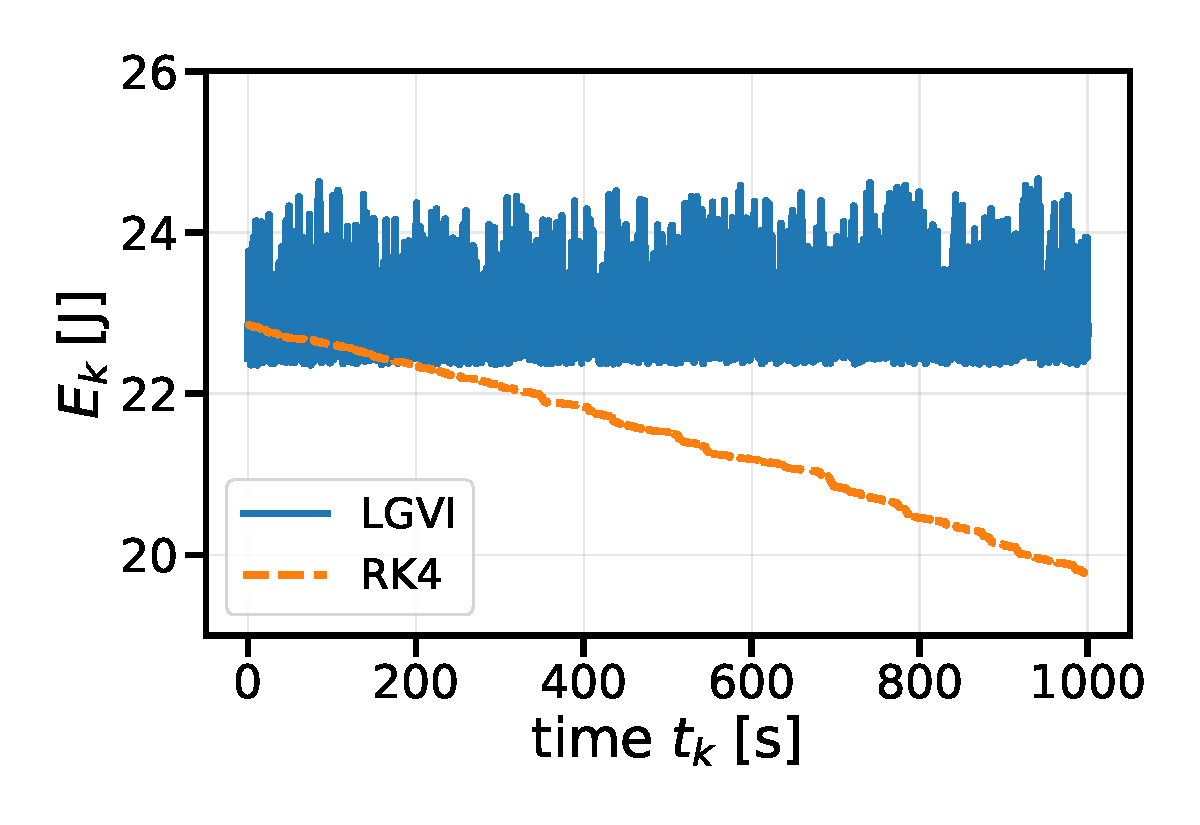
\includegraphics[width=\textwidth]{pics/Numerical_Simulation/Acrobot/acrobot_total_energy.pdf}
        \caption*{(a) Total energy $E_k$.}
    \end{minipage}
    \hfill
    \begin{minipage}{0.49\textwidth}
        \centering
        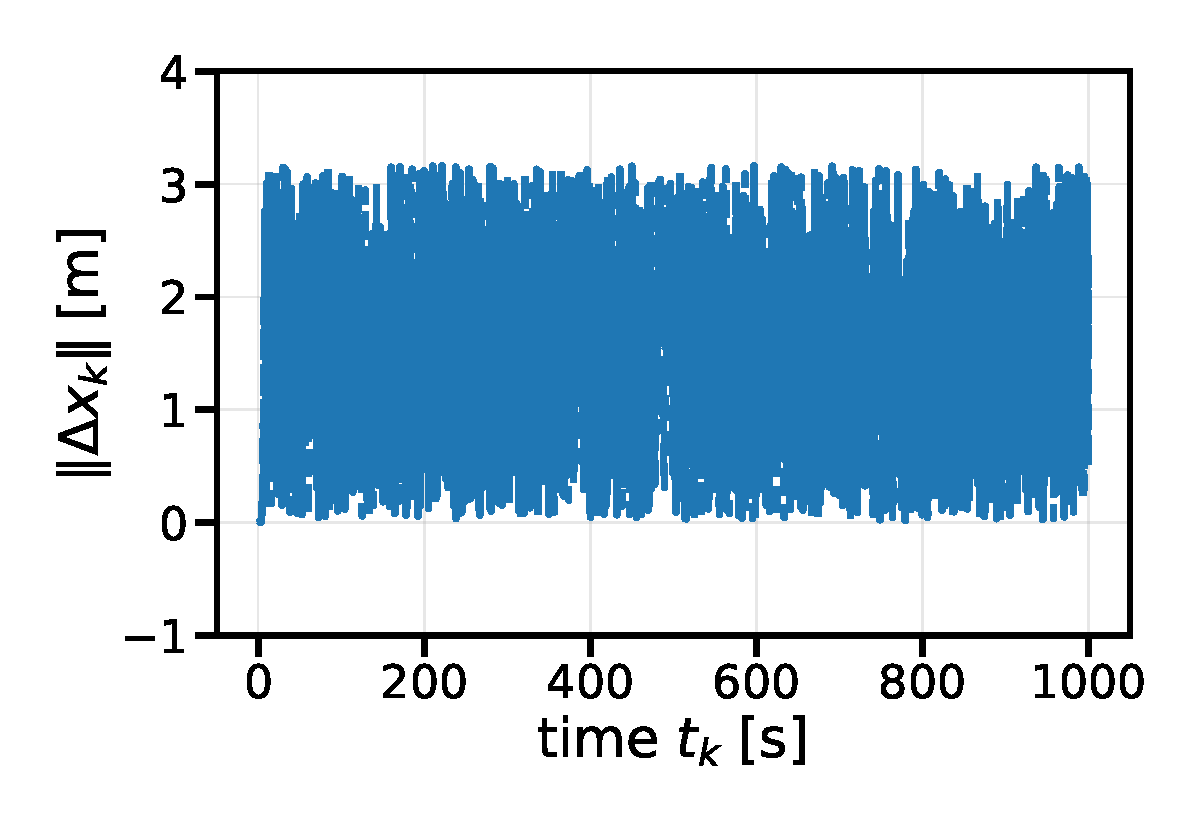
\includegraphics[width=\textwidth]{pics/Numerical_Simulation/Acrobot/acrobot_position_error_norm.pdf}
        \caption*{(b) Position error norm $\|\Delta \bm{x}_k \||$.}
    \end{minipage}

    \vspace{0.5em}

    \begin{minipage}{0.49\textwidth}
        \centering
        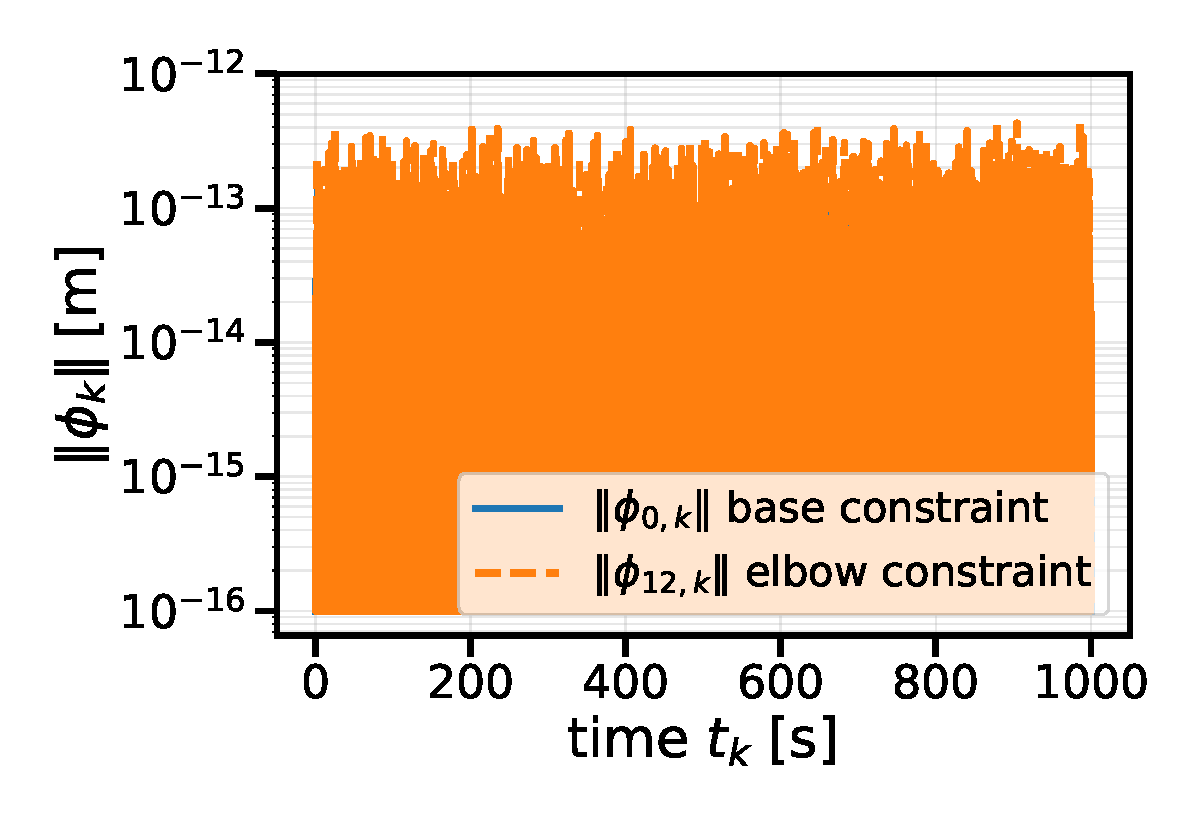
\includegraphics[width=\textwidth]{pics/Numerical_Simulation/Acrobot/acrobot_holonomic_constraint_residuals.pdf}
        \caption*{(c) Holonomic constraint residual $\bm{\phi}$.}
    \end{minipage}
    \hfill
    \begin{minipage}{0.49\textwidth}
        \centering
        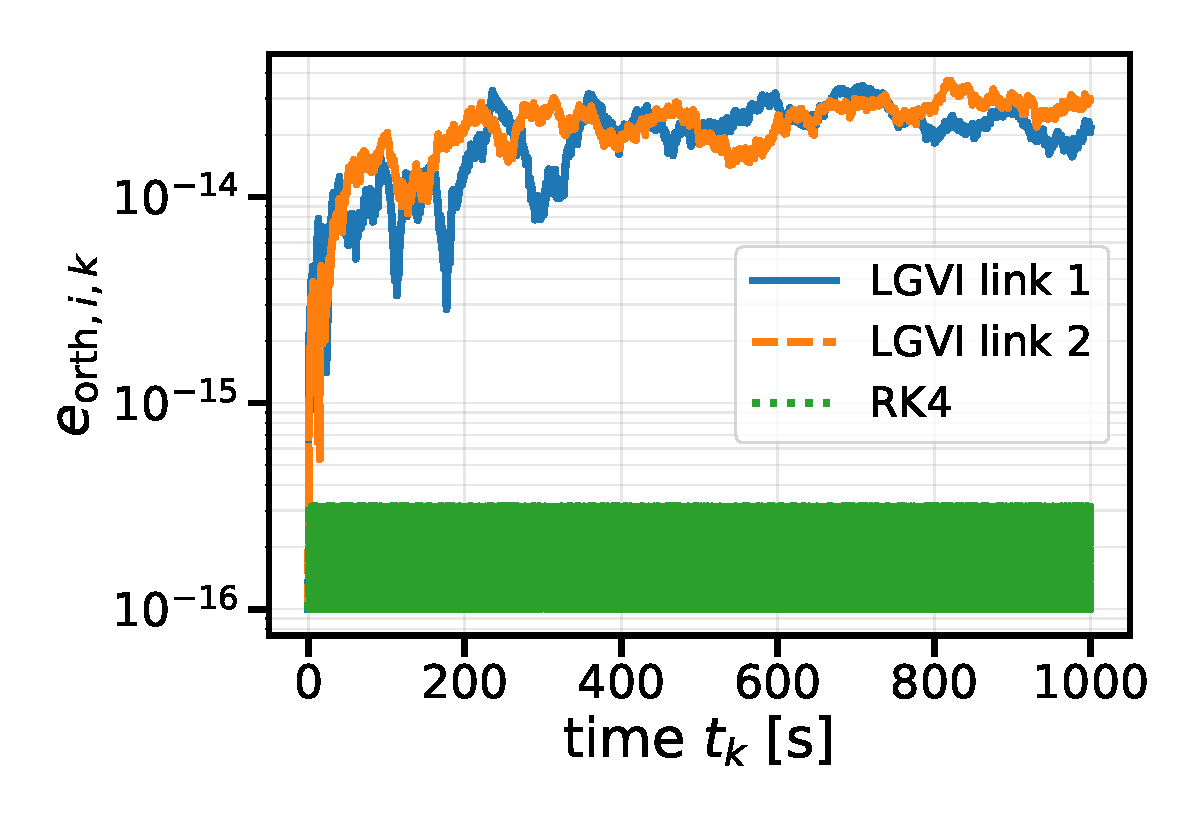
\includegraphics[width=\textwidth]{pics/Numerical_Simulation/Acrobot/acrobot_orthogonality_error.pdf}
        \caption*{(d) Orthogonality error $e_{orth}$.}
    \end{minipage}

    \caption{Comparison of the numerical preservation properties for the unforced Acrobot.}
    \label{fig:simulation_results_acrobot_unforced}
\end{figure}

The total energy $E_k$ is shown in Fig.\ref{fig:simulation_results_acrobot_unforced}(a). Since the system is unforced, the exact mechanical energy is expected to remain constant. The LGVI energy remains close to its initial value and shows bounded oscillations over the long-time horizon. This behaviour is consistent with the symplectic structure of variational integrators introduced in Section \ref{sec:properties_discrete_lagrangian_flow}. In contrast, the RK4 reference shows a visible drift of the energy over time. This agrees with the observation from the unforced 3D-pendulum simulation in Fig.\ref{fig:simulation_results_3d_pendulum}.

Fig.~\ref{fig:simulation_results_acrobot_unforced}(b) shows the position error norm
$\|\Delta \bm{x}_k\|$ between the LGVI trajectory and the reconstructed RK4
reference. It subsequently grows and oscillates over the long-time
horizon, reaching a maximum of approximately $\SI{3.16}{\meter}$. The deviation is reasoned, by
the numerical differences between the two
integrators LGVI and RK4.

The holonomic constraint residuals $\|\bm{\phi}_{0,k}\|_2$ and $\|\bm{\phi}_{12,k}\|_2$ are shown in Fig.\ref{fig:simulation_results_acrobot_unforced}(c). Both the base constraint residual $\|\bm{\phi}_{0,k}\|_2$ and the elbow constraint residual $\|\bm{\phi}_{12,k}\|_2$ remain close to machine precision over the complete simulation ($< 10^{-12}$). This confirms that the constrained LGVI in maximal-coordinates \eqref{eq:acrobot_full_del_shifted} enforces the fixed-base joint and the elbow joint at the position level.

Finally, Fig.\ref{fig:simulation_results_acrobot_unforced}(d) shows the orthogonality error $e_{orth,i,k}$ of both link rotations. The LGVI preserves the $SO(2)$ structure of both attitudes by the multiplicative update $\bm{R}_{i,k+1}=\bm{R}_{i,k}\bm{F}_{i,k}$ with $\bm{F}_{i,k}\in SO(2)$. The RK4 reference also remains very small, because it is integrated in relative coordinates and then reconstructed into rotation matrices. However, the LGVI shows a slightly larger error, which is caused by the finite tolerance of the Newton iteration used to compute the Cayley parameters. Nevertheless, the orthogonality error remains below $10^{-13}$ over the complete simulation.

Overall, the unforced Acrobot simulation confirms that the derived constrained LGVI preserves the geometric structure of the maximal-coordinate model. The link attitudes remain on $SO(2)$, the joint constraints remain satisfied, and the energy shows bounded long-time behaviour.

\subsubsection{Controlled Acrobot}

The Acrobot is actuated by a scalar torque at the elbow joint. As derived in \eqref{eq:acrobot_generalized_torque}, this torque is an internal joint torque acting between the two links.
The control input is chosen as the sinusoidal elbow torque
\[
u(t)=0.15\sin(0.7t)\,\si{\newton\meter}.
\]
The discrete input is obtained by evaluating the continuous input at the time nodes, $u_k=u(t_k)$. The forced simulation uses the same physical parameters and initial condition as the unforced case. The simulation is performed with
\[
h=\SI{0.001}{\second},
\qquad
t_f=\SI{100}{\second},
\]
corresponding to $N=100000$ discrete-time steps. The same metrics as in the unforced case are evaluated.

\begin{figure}[t]
    \centering
    \begin{minipage}{0.49\textwidth}
        \centering
        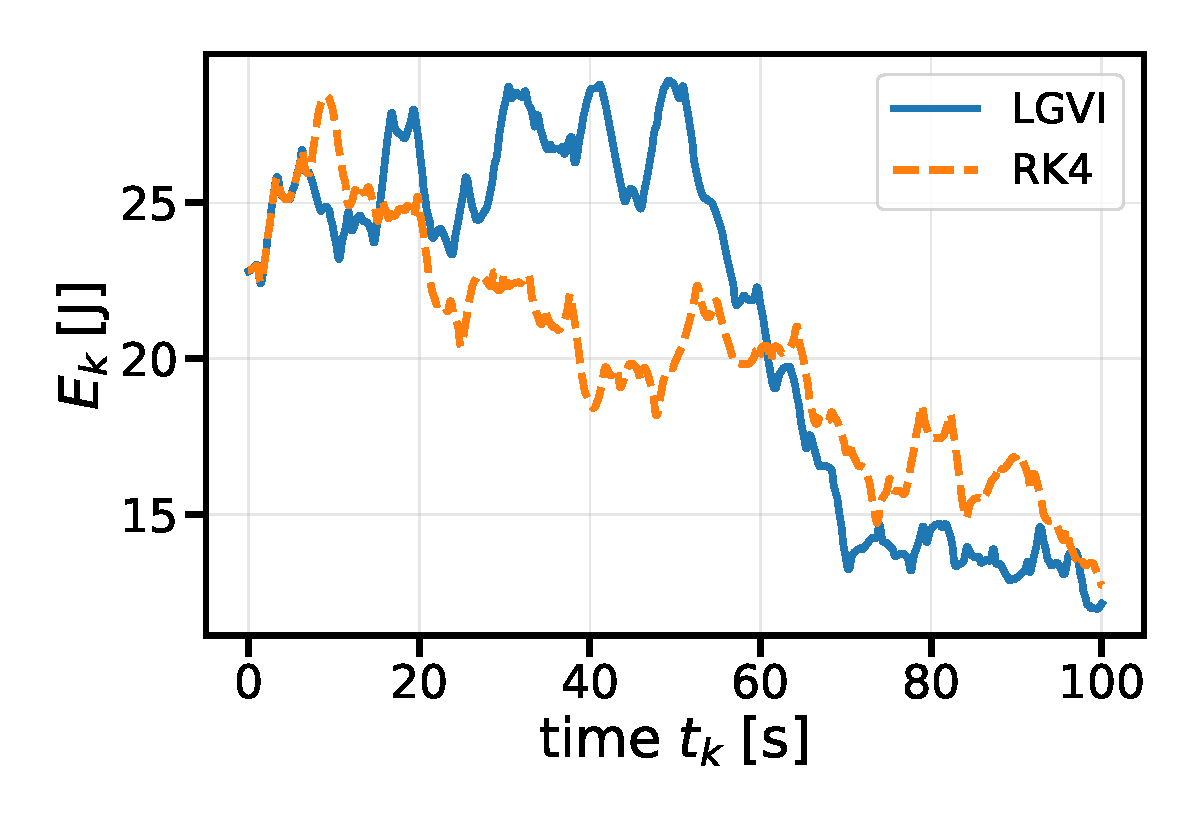
\includegraphics[width=\textwidth]{pics/Numerical_Simulation/Acrobot/forced_sine_total_energy.pdf}
        \caption*{(a) Total energy $E_k$.}
    \end{minipage}
    \hfill
    \begin{minipage}{0.49\textwidth}
        \centering
        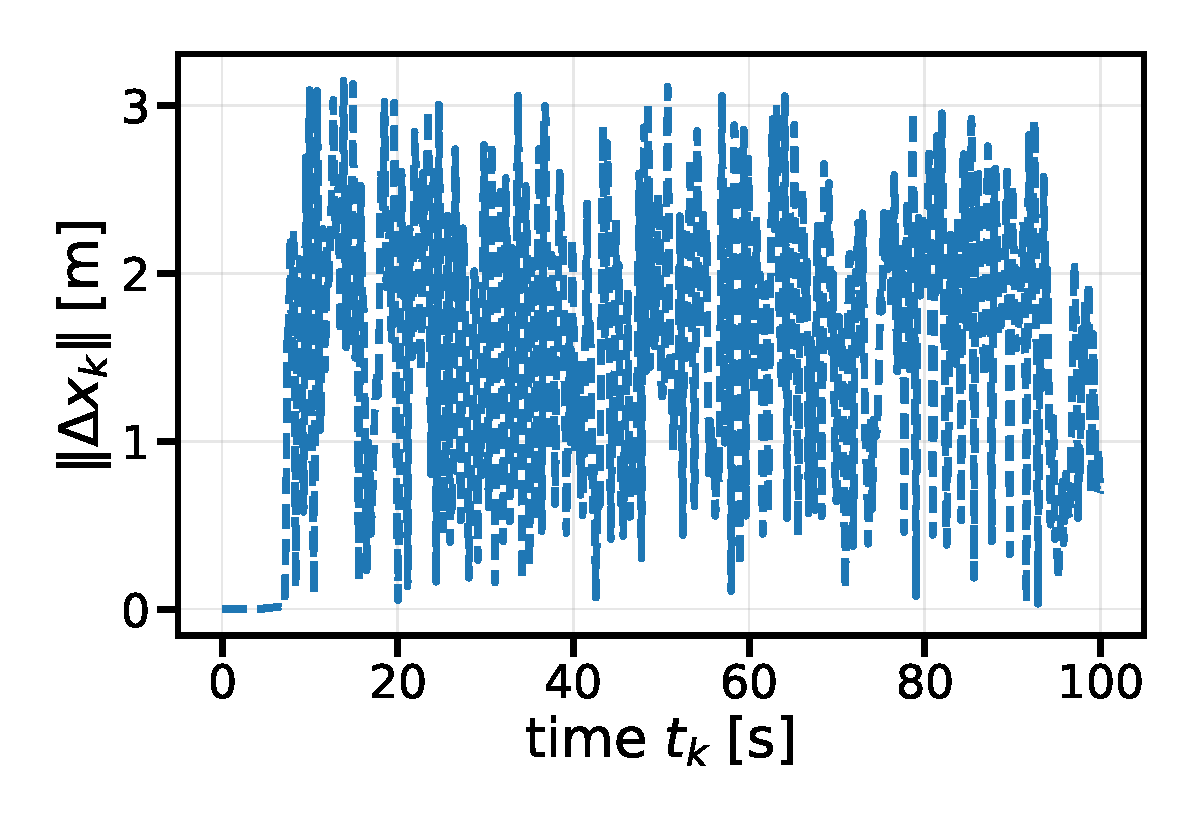
\includegraphics[width=\textwidth]{pics/Numerical_Simulation/Acrobot/forced_sine_position_error.pdf}
        \caption*{(b) Position error norm $\|\Delta \bm{x}_k \|$.}
    \end{minipage}

    \vspace{0.5em}

    \begin{minipage}{0.49\textwidth}
        \centering
        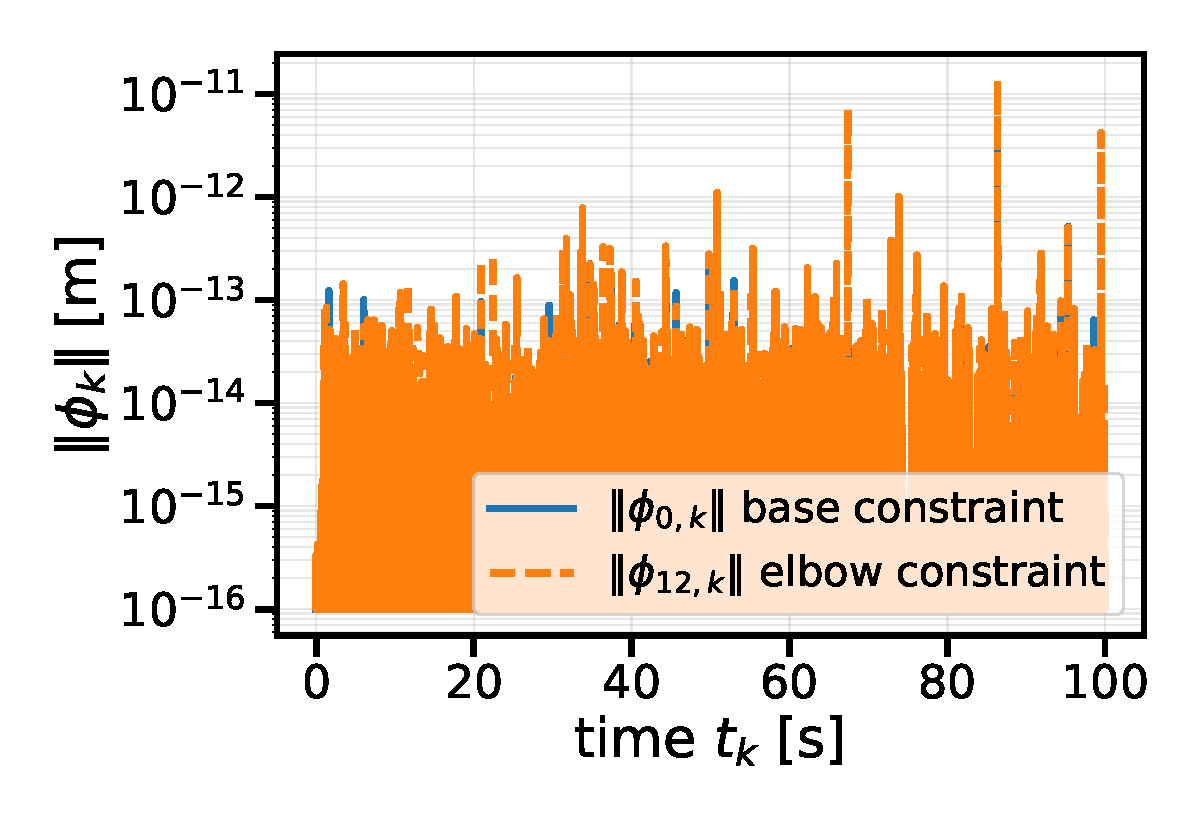
\includegraphics[width=\textwidth]{pics/Numerical_Simulation/Acrobot/forced_sine_constraint_residuals.pdf}
        \caption*{(c) Holonomic constraint residual $\bm{\phi}$.}
    \end{minipage}
    \hfill
    \begin{minipage}{0.49\textwidth}
        \centering
        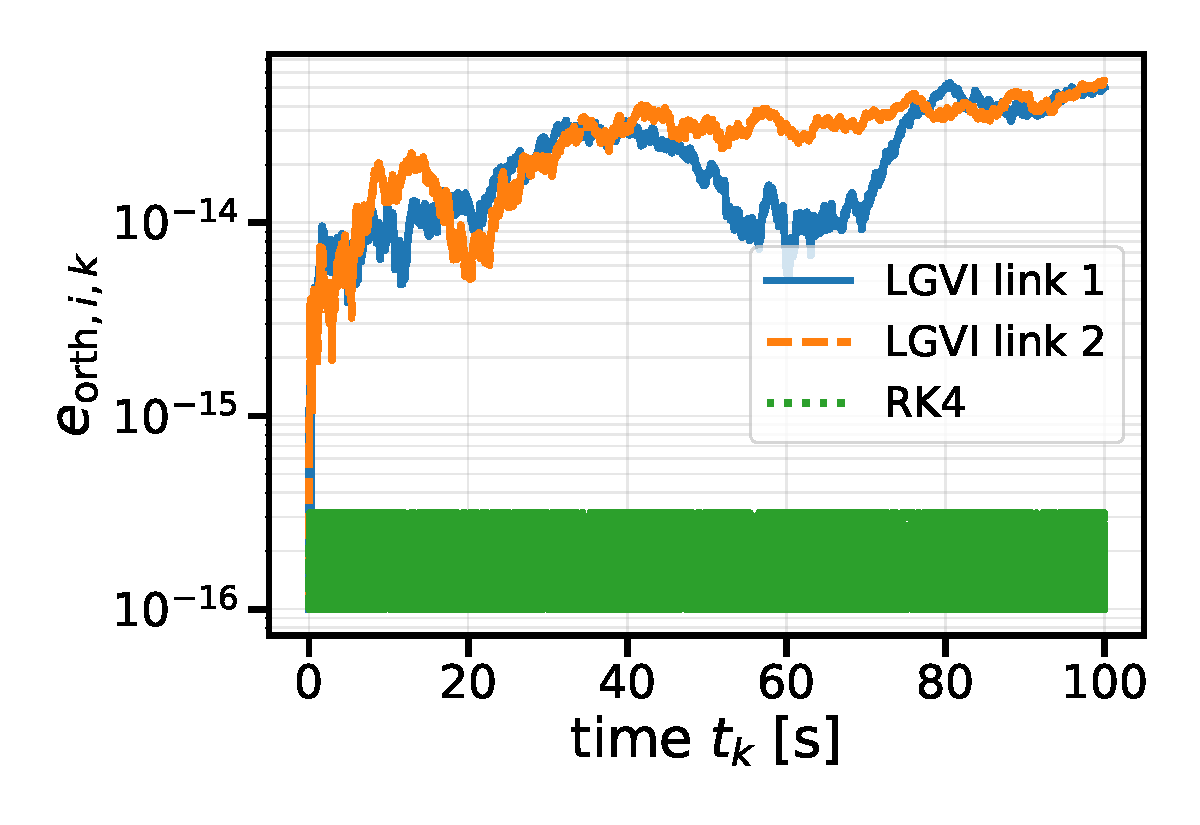
\includegraphics[width=\textwidth]{pics/Numerical_Simulation/Acrobot/forced_sine_orthogonality_error.pdf}
        \caption*{(d) Orthogonality error $e_{orth}$.}
    \end{minipage}

    \caption{Numerical simulation results for the controlled Acrobot.}
    \label{fig:simulation_results_acrobot_forced}
\end{figure}

The total energy \(E_k\) of the controlled Acrobot is shown in
Fig.~\ref{fig:simulation_results_acrobot_forced}(a). As for the controlled
3D pendulum, the LGVI and RK4 energies agree closely during approximately the
first $\SI{5}{\second}$ and subsequently deviate as the numerical trajectories
separate. In contrast to the unforced case, the applied torque performs work on
the system, and the mechanical energy is therefore neither conserved nor
expected to remain bounded around its initial value.

Fig.~\ref{fig:simulation_results_acrobot_forced}(b) shows the position error
norm $\|\Delta \bm{x}_k\|$ between the LGVI trajectory and the RK4 reference.
The error is initially zero and remains close to zero over the
first $\SI{5}{\second}$, confirming that both methods reproduce the same
short-time response to the sinusoidal elbow input. It then increases and
oscillates as the trajectories diverge, following the same
behaviour observed for the controlled 3D pendulum, because of the
numerical differences between the two methods.

The holonomic constraint residuals $\|\bm{\phi}_{0,k}\|_2$ and $\|\bm{\phi}_{12,k}\|_2$ are plotted in Fig.\ref{fig:simulation_results_acrobot_forced}(c). The base and elbow constraint residuals are negligible ($< 10^{-11}$) over the complete simulation. In the forced case, the maximal-coordinate LGVI therefore also prevents constraint drift and keeps the Acrobot links physically connected, which is essential for the later SDP optimization conducted in Section \ref{sec:acrobot_optimization_results}.

Finally, Fig.\ref{fig:simulation_results_acrobot_forced}(d) shows the orthogonality error $e_{orth,i,k}$ of both link rotations. As in the unforced simulation, the LGVI preserves the $SO(2)$ structure through the attitude update \eqref{eq:acrobot_full_del_shifted_kinematics_1} and \eqref{eq:acrobot_full_del_shifted_kinematics_2}. As in the unforced case, the RK4 reference remains close to zero, since its rotations are represented as rotation matrices. Therefore, the controlled Acrobot simulation confirms that both the forcing term and the constrained Lie-group update are numerically consistent.

Overall, Fig.~\ref{fig:simulation_results_acrobot_unforced} and
Fig.~\ref{fig:simulation_results_acrobot_forced} show that the Acrobot LGVI also behaves
consistently for a constrained multi-body system, introduced in Section \ref{sec:multi_body_systems}. The method preserves the
\(SO(2)\) structure, keeps the holonomic constraints small, and aligns closely with
the RK4 reference for the tested timestep.


\section{3D-Pendulum Optimization Results}
\label{sec:3d_pendulum_optimization_results}

This section evaluates the controlled 3D-pendulum polynomial optimization
problem (POP) \eqref{eq:controlled_3d_pendulum_pop} introduced in
Section~\ref{sec:discrete_motion_planning_3d_pendulum}. The POP is converted
into a sparse second-order Moment-SOS relaxation using SPOT and is solved with
MOSEK \cite{Kang_2025Global}. The implementation is documented in
\cite{Elshani2026CTO_GitHub}. All experiments were conducted 
on the Harvard FASRC Cannon cluster using Intel Xeon Sapphire Rapids CPUs and 
\(512\,\mathrm{GB}\) of RAM. Each optimization was executed on a 
single compute node using 8 CPU cores.

\paragraph{Optimization Configuration}
The physical parameters are identical to those used for the $3$D pendulum in
Section \ref{subsec:3d_pendulum_numercial_simulation}.
For all optimization runs, the
relaxation order, SDP time step, number of time steps, and prediction horizon
are
\begin{equation}
    \kappa=2,
    \qquad
    \Delta t_{\mathrm{SDP}}=0.1\,\mathrm{s},
    \qquad
    N=20,
    \qquad
    T=N\Delta t_{\mathrm{SDP}}=2.0\,\mathrm{s}.
    \label{eq:3d_pendulum_optimization_configuration}
\end{equation}
The initial attitude is $\bm{R}^{\mathrm{init}}=\bm{R}_x(5^\circ)$ and the initial
relative rotation is $\bm F^{\mathrm{init}}=\bm I$. Starting from the same
initial state, the desired rotation angle is varied as
\(\theta_{x,\mathrm{des}}\in
\{0^\circ,45^\circ,90^\circ,135^\circ,180^\circ\}\) around the x-axis, with
\(\bm{R}_{\mathrm{des}}=\bm{R}_x(\theta_{x,\mathrm{des}})\). The terminal 
desired relative rotation is chosen to be $\bm{F}_{\mathrm{des}}=\bm{I}$, which represents 
zero velocity at step $N$ of the 3D-pendulum.
The scalar control and relative-rotation limits of the POP are set as
\begin{align*}
    u_{\max}
    &=5,
    \\
    \cos(\Delta\theta_{\max})
    &=0.5.
\end{align*}
The objective parameters of \eqref{eq:controlled_3d_pendulum_pop_objective} 
remain constant for all target rotations and are
identical to the Acrobot optimization configuration in
Table \ref{tab:optimization_cost_parameters}.

The correlative sparsity pattern is completed with the minimum-degree (MD)
chordal-extension heuristic introduced in
Section~\ref{subsec:sparse_relaxations} \cite{Kang_2025Global}. For the present
problem, the largest clique generated by SPOT contains $24$ scalar variables.
Consequently, its order-two moment matrix has
\(\binom{24+2}{2}=325\) rows and columns. In comparison, the complete
$39$-variable temporal
chain-like clique $\bm{z}_{\mathrm{P}}(\mathcal I_k^{\mathrm{P}})$ would produce an $820\times820$ matrix, while the dense
relaxation for $N=20$ would require a
$91{,}378\times91{,}378$ matrix (see Section \ref{sec:discrete_motion_planning_3d_pendulum}).
Therefore, the MD chordal extension substantially
reduces the dense or chain-like moment-matrix in this experiment.

\paragraph{Evaluation metrics}
The angular rotation error at time step $k$ is
evaluated from the ordered SDP extraction in degrees as
\begin{equation}
    e_{R,k}^{P}
    =
    \frac{180}{\pi}\theta_{k}^{\mathrm{rad}},
    \qquad
    \theta_{k}^{\mathrm{rad}}
    =
    \cos^{-1}\!\left(
        \frac{\operatorname{tr}(\bm R_{\mathrm{des}}^\top\bm R_k)-1}{2}
    \right),
    \label{eq:3d_pendulum_evaluation_rotation_error}
\end{equation}
where $\theta_k^{\mathrm{rad}}$ is the relative rotation angle in radians and
$\bm{R}_{\mathrm{des}}^\top \bm{R}_k$ is the relative rotation to the target attitude
\cite{GallierQuaintance2020LinearAlgebra}. Thus, $e_{R,k}^{P}$ is reported in degrees.
Thereby, the terminal angular error at $N$
is denoted as $e_{R,N}^{P}$.
In addition, the maximum orthogonality violation over the optimization horizon is defined as
\begin{equation}
    e_{\mathrm{orth}}^{P,\max}
    =\max_{0\leq k\leq N}
    \left\lVert
        \bm R_k^{\top}\bm R_k-\bm I
    \right\rVert_F.
    \label{eq:3d_pendulum_evaluation_terminal_error}
\end{equation}

In order to evaluate the optimality of the lower-bound solution $\gamma_{\kappa}^*$,
a feasible upper bound $p(\widehat{\bm{z}})$ can be generated through a
nonlinear programming (NLP) solver \cite{Sangli2025}. Thereby, the corresponding 
objectives $J_{SDP}$ and $J_{NLP}$ can be calculated, whose suboptimality gap is given by 
\begin{equation}
    \epsilon
    =
    \frac{
        \left|J_{\mathrm{NLP}}-J_{\mathrm{SDP}}\right|
    }{
        \left|J_{\mathrm{NLP}}\right|+10^{-6}
    }.
    \label{eq:3d_pendulum_warm_start_gap}
\end{equation}
Here, the SDP trajectory extraction is used as a warm start for the NLP solver,
using the GitHub code of \cite{Sangli2025}. The resulting suboptimality gap is denoted by $\epsilon_{\mathrm{warm}}$.
The numerical rank condition $\delta_{\max}$ is evaluated according to
\eqref{eq:numerical_rank_metric} over the sub-moment matrices used for the
ordered extraction. The runtime given in Table \ref{tab:pendulum_3d_sdp_statistics} 
is the MOSEK optimizer time.

\begin{table}[!htbp]
    \centering
    \caption{Results of the controlled $3$D pendulum for desired $x$-axis rotations.}
    \label{tab:pendulum_3d_sdp_statistics}

    \setlength{\tabcolsep}{6pt}
    \renewcommand{\arraystretch}{1.15}

    \resizebox{\textwidth}{!}{%
    \begin{tabular}{@{}lccccc@{}}
        \toprule
        $\theta_{x,\mathrm{des}}$
        & $0^\circ$
        & $45^\circ$
        & $90^\circ$
        & $135^\circ$
        & $180^\circ$ \\
        \midrule

        Terminal angular error $e_{R,N}^{P}$
        & $0.0389^\circ$
        & $13.735^\circ$
        & $19.496^\circ$
        & $10.614^\circ$
        & $0.1418^\circ$ \\

        Manifold violation $e_{\mathrm{orth}}^{P,\max}$
        & $1.2\!\times\!10^{-9}$
        & $4.6\!\times\!10^{-8}$
        & $1.1\!\times\!10^{-11}$
        & $2.6\!\times\!10^{-9}$
        & $4.5\!\times\!10^{-8}$ \\

        Suboptimality gap $\epsilon_{warm}$
        & $1.8\!\times\!10^{-6}$
        & $8.8\!\times\!10^{-8}$
        & $5.6\!\times\!10^{-10}$
        & $2.4\!\times\!10^{-9}$
        & $2.8\!\times\!10^{-9}$ \\

        Rank condition $\delta_{\max}$
        & $3.0\!\times\!10^{-9}$
        & $7.3\!\times\!10^{-8}$
        & $1.1\!\times\!10^{-11}$
        & $3.2\!\times\!10^{-9}$
        & $2.3\!\times\!10^{-8}$ \\

        Runtime (s)
        & $3349.46$
        & $3706.36$
        & $4032.72$
        & $4128.29$
        & $3873.03$ \\
        \bottomrule
    \end{tabular}%
    }
\end{table}

\begin{figure}[t!]
    \centering
    \begin{minipage}{0.49\textwidth}
        \centering
        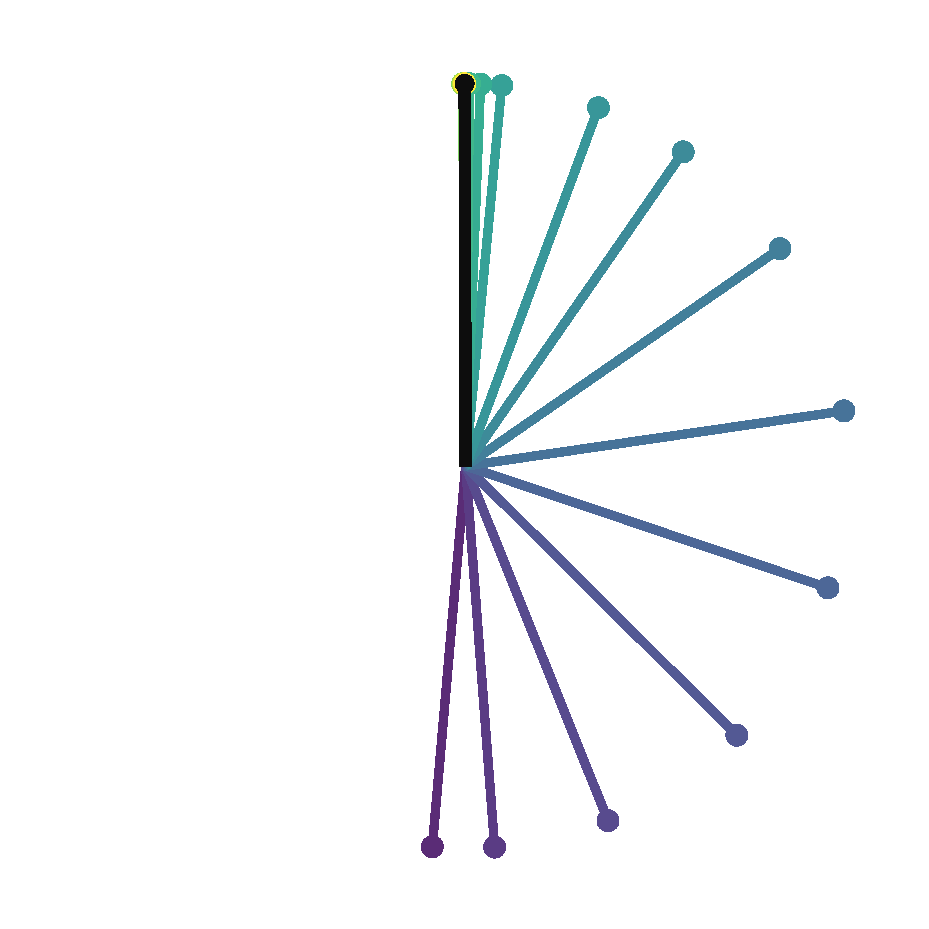
\includegraphics[width=0.70\linewidth]{pics/Optimization/3D_Pendulum/MD_180_deg_Pendulum_trajectory_matlab.pdf}
        \caption*{(a) 3D-Pendulum trajectory.}
    \end{minipage}
    \hfill
    \begin{minipage}{0.49\textwidth}
        \centering
        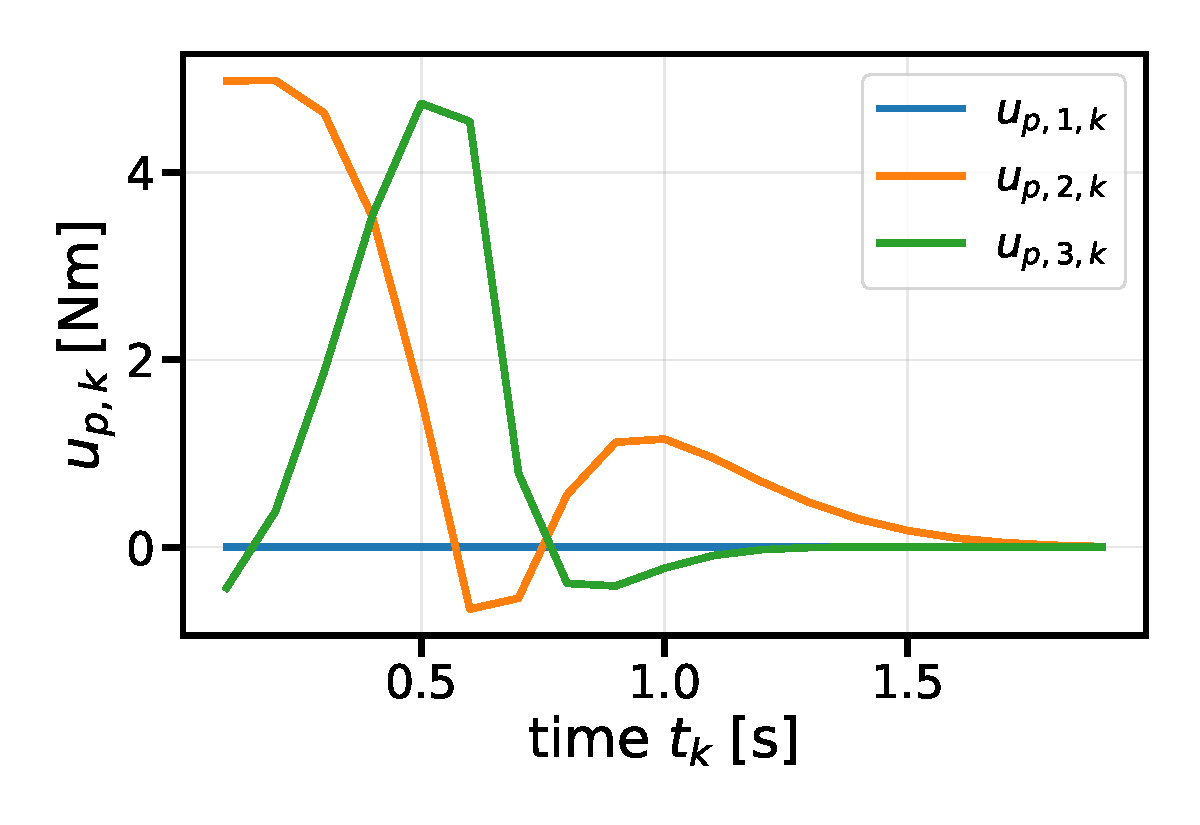
\includegraphics[width=\linewidth]{pics/Optimization/3D_Pendulum/MD_180_deg_Pendulum_control_input.pdf}
        \caption*{(b) Control inputs $\bm u_{p,k}$.}
    \end{minipage}

    \vspace{0.5em}

    \begin{minipage}{0.49\textwidth}
        \centering
        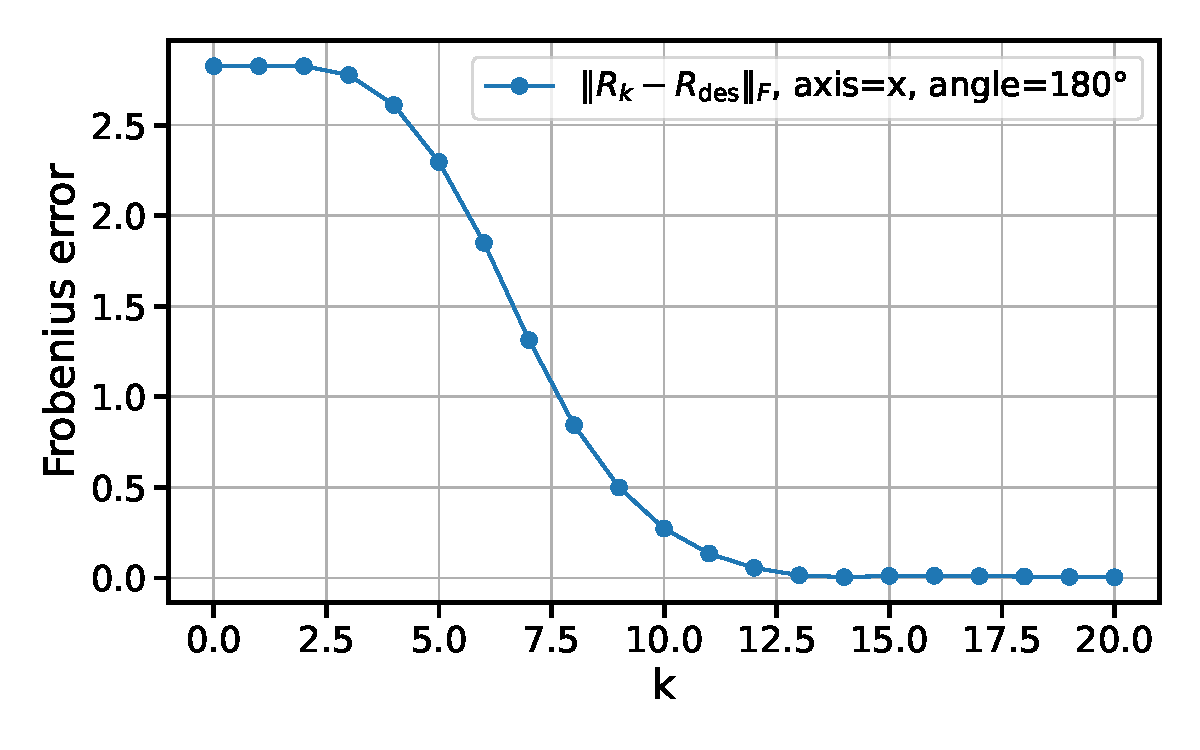
\includegraphics[width=\linewidth]{pics/Optimization/3D_Pendulum/MD_180_deg_Pendulum_frobenius.pdf}
        \caption*{(c) Angular rotation tracking error $e_{R,k}^{P}$.}
    \end{minipage}
    \hfill
    \begin{minipage}{0.49\textwidth}
        \centering
        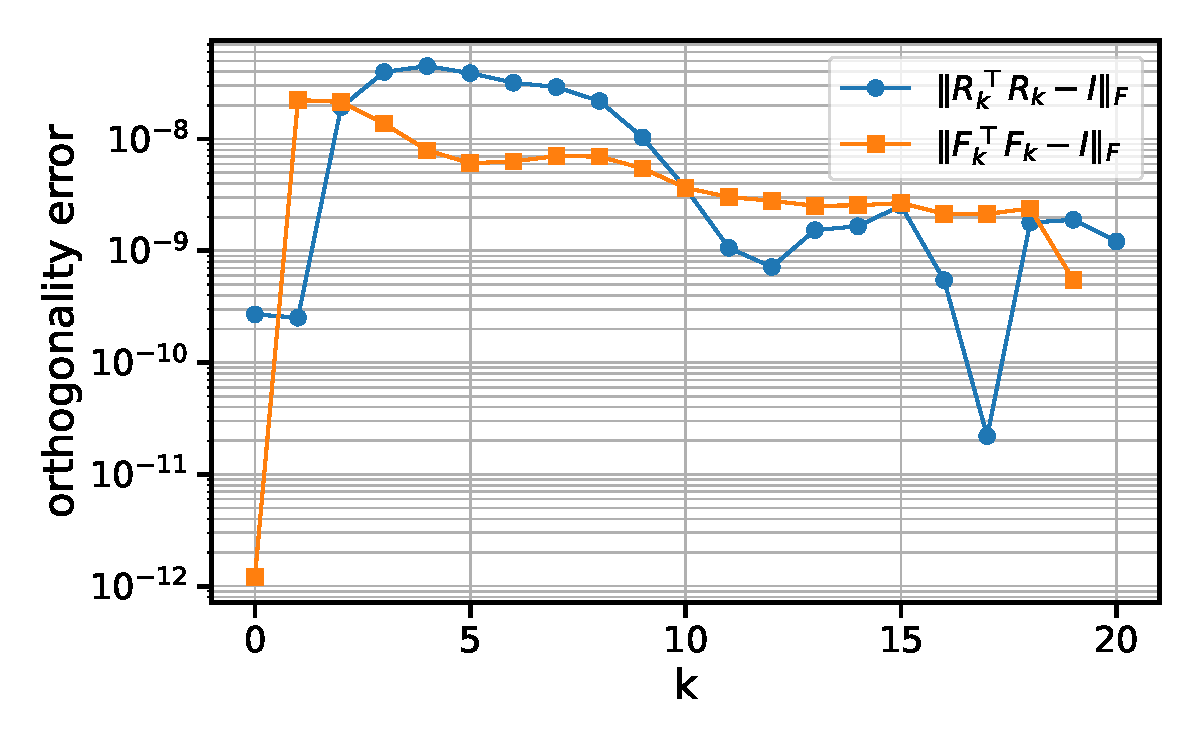
\includegraphics[width=\linewidth]{pics/Optimization/3D_Pendulum/MD_180_deg_Pendulum_orthogonality.pdf}
        \caption*{(d) Orthogonality errors $e_{\mathrm{orth},k}^{P}$ of
        $\bm R_k$, $\bm F_k$.}
    \end{minipage}

    \caption{SPOT optimization results for the controlled $3$D pendulum
    performing a $180^\circ$ rotation about the $x$-axis using the MD
    sparsity setting: (a) optimization trajectory,
    (b) control inputs
    $\bm u_{p,k}$, (c) angular rotation tracking error $e_{R,k}^{P}$, and
    (d) orthogonality errors $e_{\mathrm{orth},k}^{P}$}
    \label{fig:optimization_results_x180_md}
\end{figure}

\paragraph{Results}

Table~\ref{tab:pendulum_3d_sdp_statistics} shows that 
\(e_{\mathrm{orth}}^{P,\max}\leq4.6\times10^{-8}\) for all target rotations. Therefore, the 
extracted rotation matrices satisfy the orthogonality constraints. 
Moreover, \(\epsilon_{\mathrm{warm}}\leq1.8\times10^{-6}\) and 
\(\delta_{\max}\leq7.3\times10^{-8}\). The feasible NLP upper bounds and the SDP lower 
bounds therefore nearly coincide, while the maximal rank condition $\delta_{\max}$ of the 
evaluated sub-moment matrices is numerically 
close to rank one. Consequently, the suboptimality gap $\epsilon_{\mathrm{warm}}$ 
and rank metric validate the tightness
of the second-order MD relaxation for the considered 3D-pendulum test cases,
certifying the feasibility of the extracted solutions.

The terminal angular error does not increase monotonically with the target rotation
\(\theta_{x,\mathrm{des}}\). The smallest errors are obtained for the \(0^\circ\) and 
\(180^\circ\) targets, with \(e_{R,N}^{P}=0.0389^\circ\) and 
\(e_{R,N}^{P}=0.1418^\circ\). In contrast, the intermediate targets 
result in errors of \(13.735^\circ\), \(19.496^\circ\), and \(10.614^\circ\) for 
\(45^\circ\), \(90^\circ\), and \(135^\circ\). Consequently, the \(90^\circ\) target 
produces the largest terminal tracking error. The reason for this behaviour is that
the corresponding POP \eqref{eq:controlled_3d_pendulum_pop} does not require the 
optimal trajectory to reach the desired attitude exactly, as $\bm{R}_{\mathrm{des}}$ is not considered
as a hard terminal constraint but weighted in the objective. Furthermore, the \(0^\circ\) and 
\(180^\circ\) attitudes are equilibrium configurations of the considered pendulum for which 
the gravitational moment vanishes. In contrast, the intermediate attitudes require a 
control moment to stay at $\bm{R}_{\mathrm{des}}$, which contributes to their larger terminal errors. 

Fig.\ref{fig:optimization_results_x180_md} illustrates the ordered extraction 
for a desired rotation of \(\theta_{x,\mathrm{des}}=180^\circ\). The 
optimized trajectory follows a smooth path
from the initial to the inverted configuration.
As the rotation is around the x-axis, \(u_{p,1,k}\) 
remains zero. When reaching the final horizon time at $T=\SI{2}{\second}$, all three control
inputs approach zero. Correspondingly, the angular tracking error \(e_{R,k}^{P}\)
decreases from approximately \(175^\circ\) and reaches \(0.1418^\circ\) at the terminal time.
Finally, the orthogonality errors of both \(\bm R_k\) and \(\bm F_k\) remain less then
\(10^{-8}\), which validates the feasibility of the extracted solution. 
The four panels therefore show that the extracted trajectory performs the 
desired rotational motion while remaining on the Lie group.

\section{Acrobot Optimization Results}
\label{sec:acrobot_optimization_results}

This section evaluates the controlled Acrobot polynomial optimization problem
(POP) introduced in Section~\ref{sec:discrete_motion_planning_acrobot}. As for
the $3$D pendulum, SPOT constructs a sparse
second-order Moment-SOS relaxation, which is solved using MOSEK \cite{Kang_2025Global}. First, the
semidefinite optimization of
Section \ref{sec:trajectory_optimization_via_sdp_relaxation} is investigated.
For the larger desired rotations, its ordered extraction does not provide a
certified feasible trajectory over the complete horizon. This motivates the
closed-loop SDP--MPC formulation of
Section \ref{sec:acrobot_trajectory_optimization_SDP_MPC}, which applies only
the first extracted control before solving the problem again. The complete
implementation is documented in \cite{Elshani2026CTO_GitHub}. All experiments were conducted 
on the Harvard FASRC Cannon cluster using Intel Xeon Sapphire Rapids CPUs and 
\(512\,\mathrm{GB}\) of RAM. Each optimization was executed on a 
single compute node using 8 CPU cores.

\subsection{Semidefinite Optimization Results}
\label{subsec:acrobot_optimization_results}

\paragraph{Optimization configuration}
The physical parameters are identical to those of the Acrobot simulation in
Section~\ref{subsec:evaluation_acrobot}. For all optimization runs, the
relaxation order, SDP time step, and number of time steps are
\begin{equation}
    \kappa=2,
    \qquad
    \Delta t_{\mathrm{SDP}}=0.1\,\mathrm{s},
    \qquad
    N=60,
    \qquad
    N\Delta t_{\mathrm{SDP}}=6.0\,\mathrm{s}.
    \label{eq:acrobot_sdp_optimization_configuration}
\end{equation}
The complete discretization window from the history node $k=0$ to the terminal
node $k=N$ therefore spans $6.0\,\mathrm{s}$.

Both links start from the same initial attitude and relative rotation,
\begin{equation}
    \bm R_1^{\mathrm{init}}
    =\bm R_2^{\mathrm{init}}
    =\bm R(5^\circ),
    \qquad
    \bm F_1^{\mathrm{init}}
    =\bm F_2^{\mathrm{init}}
    =\bm I,
    \label{eq:acrobot_sdp_initial_configuration}
\end{equation}
where $\bm R(\theta)\in SO(2)$ denotes the planar rotation matrix defined in
\eqref{eq:so2_rotation_matrix}. Starting from this state, the same desired
absolute rotation is assigned to both links
\begin{equation}
    \theta_1^{\mathrm{des}}
    =\theta_2^{\mathrm{des}}
    =\theta_{\mathrm A}^{\mathrm{des}}
    \in
    \{0^\circ,45^\circ,90^\circ,135^\circ,180^\circ\},
    \label{eq:acrobot_sdp_target_configurations}
\end{equation}
with desired relative rotation $\bm F_1^{\mathrm{des}}
    =\bm F_2^{\mathrm{des}}
    =\bm I_2$ after $N=60$.
In particular, $\theta_{\mathrm A}^{\mathrm{des}}=180^\circ$ represents the inverted
equilibrium with both links at rest, which is considered as a final stabilization target for the Acrobot.
The physical control and multiplier scales
of \eqref{eq:acrobot_variable_scaling}, together with the link-specific rotation
increment bounds in \eqref{eq:controlled_acrobot_pop_step_bound}, are chosen as
\begin{equation}
    u_{\max}=15\,\mathrm{N\,m},
    \qquad
    \lambda_{\max}=40\,\mathrm{N},
    \qquad
    \Delta\theta_{1,\max}=70^\circ,
    \qquad
    \Delta\theta_{2,\max}=60^\circ.
    \label{eq:acrobot_sdp_optimization_bounds}
\end{equation}
Thus, the polynomial step constraints are
$a_{1,k}\geq\cos(70^\circ)\approx0.3420$ and
$a_{2,k}\geq\cos(60^\circ)=0.5$ for $k=1,\ldots,N-1$. The objective parameters of the 
cost function \eqref{eq:controlled_acrobot_pop_objective} are summarized in
Table~\ref{tab:optimization_cost_parameters}.

\begin{table}[!htbp]
    \centering
    \caption{Objective parameters used for the $3$D-pendulum and Acrobot
    optimization experiments.}
    \label{tab:optimization_cost_parameters}
    \setlength{\tabcolsep}{12pt}
    \renewcommand{\arraystretch}{1.15}
    \begin{tabular}{@{}ccccc@{}}
        \toprule
        $w_R$ & $w_F$ & $\alpha_R$ & $\alpha_F$ & $w_u$ \\
        \midrule
        $20$ & $8$ & $15$ & $2$ & $0.09$ \\
        \bottomrule
    \end{tabular}
\end{table}

Two user-defined clique constructions are compared. The first follows the
complete chain-like sparsity of
\eqref{eq:acrobot_full_self_initial_clique}--\eqref{eq:acrobot_full_self_interior_cliques}.
At $\kappa=2$, its first clique
$\bm{z}_{\mathrm{A}}(\mathcal I_1^{\mathrm{A}})$ produces a $351\times351$ moment
matrix, while every subsequent complete clique
$\bm{z}_{\mathrm{A}}(\mathcal I_k^{\mathrm{A}})$ produces a
$253\times253$ matrix, as given in
\eqref{eq:acrobot_full_self_moment_sizes}. The second construction uses the
special multi-body sparsity in \eqref{eq:acrobot_hybrid_self_cliques}. It keeps
the complete cliques $\bm{z}_{\mathrm{A}}(\mathcal I_1^{\mathrm{A}})$ and
$\bm{z}_{\mathrm{A}}(\mathcal I_2^{\mathrm{A}})$,
but separates the later coupled dynamics
$\bm{z}_{\mathrm{A}}(\mathcal I_{\mathrm{dyn},k}^{\mathrm{A}})$ and kinematics
$\bm{z}_{\mathrm{A}}(\mathcal I_{\mathrm{kin},k}^{\mathrm{A}})$ into moment matrices
of size $171\times171$ and $91\times91$
\eqref{eq:acrobot_hybrid_self_moment_sizes}. Consequently,
the larger cliques around the first control decision are preserved, whereas the
semidefinite blocks over the remaining horizon are reduced.

\paragraph{Evaluation metrics}
Similar to the $3$D-pendulum evaluation \eqref{eq:3d_pendulum_evaluation_rotation_error}, the terminal attitude error is
reported in degrees. The combined
angular error of both links is defined as
\begin{equation}
\begin{aligned}
e_{R,k}^{\mathrm A}
&:=
\frac{180^\circ}{\pi}
\left(
    \sum_{i=1}^{2}
    \left(\theta_{i,k}^{\mathrm{rad}}\right)^2
\right)^{1/2},
\\
\theta_{i,k}^{\mathrm{rad}}
&:=
\cos^{-1}\!\left(
\frac{
\operatorname{tr}\!\left(
(\bm R_i^{\mathrm{des}})^\top
\bm R_{i,k}
\right)
}{2}
\right),
\end{aligned}
\label{eq:acrobot_terminal_rotation_error}
\end{equation}
for $i\in\{1,2\}$.
The angular error $e_{R,k}^{\mathrm A}$ is the Euclidean combination of the two
link-wise angular errors. Thereby, $e_{R,N}^{\mathrm A}$ is interpreted as a
terminal matrix error at $k=N$.
The maximum orthogonality violation is evaluated over the configuration of both links by
\begin{equation}
\begin{aligned}
    e_{\mathrm{orth}}^{\mathrm A,\max}
    =\max_{\substack{i\in\{1,2\}\\0\leq k\leq N-1}}
    \left\|
        \bm R_{i,k}^{\top}\bm R_{i,k}-\bm I_2
    \right\|_F.
\end{aligned}
\label{eq:acrobot_max_orthogonality_error}
\end{equation}
The relative-rotation errors of $\bm{F}_{i,k}$ are smaller than $\bm{R}_{i,k}$ for all $k$.
Therefore, the orthogonality of $\bm{F}_{i,k}$ is not evaluated.

The maximum numerical rank condition $\delta_{\max}$ is evaluated according to
\eqref{eq:numerical_rank_metric}~\cite{Sangli2025}. Additionally, the rank condition
of the first moment matrix, which belongs to the
clique vector \(\bm{z}_{\mathrm{A}}(\mathcal I_1^{\mathrm{A}})\), is denoted by
\begin{equation}
    \delta_1
    :=
    \frac{\nu_{2,1}}{\nu_{1,1}},
    \qquad
    \nu_{1,1}\geq\nu_{2,1}\geq0.
    \label{eq:acrobot_first_clique_rank_metric}
\end{equation}
Here, $\nu_{1,1}$ and $\nu_{2,1}$ are the two largest eigenvalues of
the moment matrix associated with
\(\bm{z}_{\mathrm{A}}(\mathcal I_1^{\mathrm{A}})\). The quantity
\(\delta_1\) is reported in addition to \(\delta_{\max}\) because
\(\bm{z}_{\mathrm{A}}(\mathcal I_1^{\mathrm{A}})\) contains the first normalized control
$\bar u_1$ used later by the subsequent MPC controller.

In contrast to the $3$D pendulum, the extracted SDP trajectories for the
Acrobot POP with $N=60$ were not certifiable for all targets. Therefore,
cold-start NLP upper bounds were generated instead of using the SDP extraction
as a warm start. The reported suboptimality gap
$\epsilon_{\mathrm{cold}}$ is computed according to
\eqref{eq:3d_pendulum_warm_start_gap} with the cold-start NLP objective. The
runtimes in Tables~\ref{tab:acrobot_sdp_statistics_full} and
\ref{tab:acrobot_sdp_statistics_hybrid} are the solver operation times reported
by the implementation.

\begin{table}[H]
    \centering
    \caption{Results of the Acrobot trajectory optimization using the
    complete chain-like cliques
    \(\bm{z}_{\mathrm{A}}(\mathcal I_k^{\mathrm{A}})\). All trajectory metrics are
    evaluated from the
    ordered extraction.}
    \label{tab:acrobot_sdp_statistics_full}
    \setlength{\tabcolsep}{6pt}
    \renewcommand{\arraystretch}{1.15}
    \resizebox{\textwidth}{!}{%
    \begin{tabular}{@{}lccccc@{}}
        \toprule
        $\theta_1^{\mathrm{des}}=\theta_2^{\mathrm{des}}$
        & $0^\circ$ & $45^\circ$ & $90^\circ$ & $135^\circ$ & $180^\circ$ \\
        \midrule
        Terminal angular error $e_{R,N}^{\mathrm A}$
        & $3.2815^\circ$
        & $54.975^\circ$
        & $64.629^\circ$
        & $36.377^\circ$
        & $3.1\!\times\!10^{-4}\,{}^\circ$ \\
        Manifold violation $e_{\mathrm{orth}}^{\mathrm A,\max}$
        & $2.2\!\times\!10^{-8}$ & $1.9\!\times\!10^{-8}$
        & $1.0368$ & $1.3688$ & $1.4053$ \\
        Suboptimality gap $\epsilon_{\mathrm{cold}}$
        & $2.0\!\times\!10^{-6}$ & $4.8\!\times\!10^{-10}$
        & $0.0717$ & $0.4126$ & $0.5233$ \\
        Rank condition $\delta_{\max}$
        & $1.4\!\times\!10^{-8}$ & $1.1\!\times\!10^{-8}$
        & $0.3542$ & $0.4696$ & $0.5596$ \\
        Rank condition $\delta_1$
        & $3.1\!\times\!10^{-9}$ & $2.8\!\times\!10^{-10}$
        & $0.003747$ & $0.1020$ & $0.2066$ \\
        Runtime $[\mathrm{s}]$
        & $2675.54$ & $3581.13$ & $6806.96$ & $5913.05$ & $5421.42$ \\
        \bottomrule
    \end{tabular}%
    }
\end{table}

\begin{table}[H]
    \centering
    \caption{Results of the Acrobot trajectory optimization using the
    special multi-body clique construction
    \(\bm{z}_{\mathrm{A}}(\mathcal I_1^{\mathrm{A}})\),
    \(\bm{z}_{\mathrm{A}}(\mathcal I_2^{\mathrm{A}})\),
    \(\bm{z}_{\mathrm{A}}(\mathcal I_{\mathrm{dyn},k}^{\mathrm{A}})\), and
    \(\bm{z}_{\mathrm{A}}(\mathcal I_{\mathrm{kin},k}^{\mathrm{A}})\).
    All metrics are defined as in
    Table~\ref{tab:acrobot_sdp_statistics_full}.}
    \label{tab:acrobot_sdp_statistics_hybrid}
    \setlength{\tabcolsep}{6pt}
    \renewcommand{\arraystretch}{1.15}
    \resizebox{\textwidth}{!}{%
    \begin{tabular}{@{}lccccc@{}}
        \toprule
        $\theta_1^{\mathrm{des}}=\theta_2^{\mathrm{des}}$
        & $0^\circ$ & $45^\circ$ & $90^\circ$ & $135^\circ$ & $180^\circ$ \\
        \midrule
        Terminal angular error $e_{R,N}^{\mathrm A}$
        & $3.2815^\circ$
        & $54.975^\circ$
        & $65.192^\circ$
        & $36.378^\circ$
        & $3.6\!\times\!10^{-4}\,{}^\circ$ \\
        Manifold violation $e_{\mathrm{orth}}^{\mathrm A,\max}$
        & $3.0\!\times\!10^{-12}$ & $3.4\!\times\!10^{-6}$
        & $1.0225$ & $1.4103$ & $1.4561$ \\
        Suboptimality gap $\epsilon_{\mathrm{cold}}$
        & $1.1\!\times\!10^{-10}$ & $9.2\!\times\!10^{-9}$
        & $0.0778$ & $0.4500$ & $0.5668$ \\
        Rank condition $\delta_{\max}$
        & $2.1\!\times\!10^{-12}$ & $2.4\!\times\!10^{-6}$
        & $0.4216$ & $0.4046$ & $0.6603$ \\
        Rank condition $\delta_1$
        & $2.6\!\times\!10^{-13}$ & $2.4\!\times\!10^{-8}$
        & $0.0010$ & $0.0973$ & $0.2172$ \\
        Runtime $[\mathrm{s}]$
        & $904.83$ & $1058.08$ & $1356.14$ & $1524.25$ & $1869.36$ \\
        \bottomrule
    \end{tabular}%
    }
\end{table}

\paragraph{Results}

Tables~\ref{tab:acrobot_sdp_statistics_full} and
\ref{tab:acrobot_sdp_statistics_hybrid} show the same qualitative behavior for
both clique constructions. For the $0^\circ$ and $45^\circ$ targets,
$\delta_{\max}$ and $e_{\mathrm{orth}}^{\mathrm A,\max}$ remain of
order $10^{-6}$. Moreover, all corresponding cold-start suboptimality gaps
satisfy $\epsilon_{\mathrm{cold}}\leq2.0\times10^{-6}$. Thus, the feasible NLP
upper bounds and the SDP lower bounds nearly coincide, while the evaluated
moment matrices are numerically close to rank one. The extracted matrices
satisfy the $SO(2)$ constraints up to a small tolerance. Together, these
metrics provide strong numerical evidence that the second-order relaxations
are tight and provide a certificate for these two cases.

The complete chain-like and special multi-body constructions give combined
terminal angular errors of $54.975^\circ$ for the $45^\circ$ target, 
This comparatively large
terminal error does not contradict the observed tightness because the desired
attitudes are included as objective terms and are not imposed as terminal
constraints. Similar to the $3$D pendulum results in
Section~\ref{sec:3d_pendulum_optimization_results}, this target is 
not an equilibrium configuration of the Acrobot.

For desired rotations of $90^\circ$, $135^\circ$, and $180^\circ$, the
definition of chain-like cliques gives terminal angular errors of $64.629^\circ$,
$36.377^\circ$, and
$3.1449\!\times\!10^{-4}\,{}^\circ$. The corresponding values
for the special multi-body construction are $65.192^\circ$,
$36.378^\circ$, and
$3.6388\!\times\!10^{-4}\,{}^\circ$. However, these terminal orientation
errors alone do not establish feasibility.

For these three targets, the values of $\delta_{\max}$ lie between $0.3542$
and $0.6603$, while $e_{\mathrm{orth}}^{\mathrm A,\max}$ lies between
$1.0225$ and $1.4561$. Consequently, the raw ordered extraction does
not represent a feasible $SO(2)$ trajectory over the complete horizon, and the
rank-one condition does not provide tightness. In particular, the 
$180^\circ$ results illustrate why both metrics must be considered together.
Although the projected terminal angular error is below
$4\!\times\!10^{-4}\,{}^\circ$, it has the highest
suboptimality gap and the largest manifold violation among all target rotations.

The cold-start NLP solutions provide
valid upper bounds for these cases. Nevertheless, the suboptimality gaps 
$\epsilon_{\mathrm{cold}}$ are
$0.0717$ and $0.0778$ for the $90^\circ$ target, $0.4126$ and $0.4500$ for
the $135^\circ$ target, and $0.5233$ and $0.5668$ for the $180^\circ$ target
for the complete chain-like and special multi-body constructions.
These large suboptimality gaps alone do not prove that the relaxation
is non-tight as it may also be a result of a suboptimal NLP upper bound \cite{Sangli2025}.
However, the higher-rank moment matrices and infeasible ordered
extractions show that global optimality is not certified for
these three cases.

Nevertheless, $\delta_1$ is smaller than $\delta_{\max}$ in every test case.
For example, the $90^\circ$ target gives $\delta_1=0.0037$
compared with $\delta_{\max}=0.3542$ for the chain-like cliques. Moreover, the 
special multi-body clique construction gives $\delta_1=0.0010$ compared with 
$\delta_{\max}=0.4216$. Consequently, the first
moment block is considerably closer to rank one than $\delta_{\max}$,
even if the moment blocks with values between $0.10$ and
$0.22$ for the $135^\circ$ and $180^\circ$ targets are generally not rank one.


The special multi-body construction produces terminal, manifold,
suboptimality-gap, and rank metrics that are comparable to the complete
chain-like construction, while its runtime is approximately $3$ to $5$
times smaller. Therefore, it is used for the following closed-loop evaluation
in Section \ref{subsec:acrobot_sdp_mpc_results}.



\subsection{Model Predictive SDP Control Results}
\label{subsec:acrobot_sdp_mpc_results}

The open-loop results of
Section~\ref{subsec:acrobot_optimization_results} show that the first-clique
rank metric $\delta_1$ is substantially smaller than the worst rank metric
$\delta_{\max}$ for all test cases (see Table \ref{tab:acrobot_sdp_statistics_hybrid}).
This observation motivates the SDP-MPC formulation of
Section~\ref{sec:acrobot_trajectory_optimization_SDP_MPC}. At every MPC
iteration, the second-order sparse Moment-SOS relaxation of the Acrobot
POP~\eqref{eq:controlled_acrobot_pop} is solved, only the first extracted control
$u_j$ in \eqref{eq:acrobot_mpc_applied_control} is applied, and the numerical
LGVI dynamics \eqref{eq:acrobot_full_del_shifted} 
are propagated (see Section \ref{subsec:evaluation_acrobot}).
The remaining predicted trajectory is ignored and the boundary data are
updated from the simulated state before the next SDP is solved. The purpose of
the following experiments is to determine whether this repeated first-step
extraction can stabilize the Acrobot at the inverted equilibrium of 
\begin{align}\label{eq:acrobot_stabilization_target}
    \theta_{\mathrm A}^{\mathrm{des}} = 180^\circ,
    \qquad
    \bm{F}^{des}_1=\bm{F}^{des}_2=\bm{I},
\end{align}
even when the
complete predicted SDP trajectory is not certifiable.

\paragraph{MPC configuration for $u_{\max}=5\,\mathrm{N\,m}$}
The physical Acrobot parameters are identical to those used for the numerical
simulation in Section~\ref{subsec:evaluation_acrobot}, and the objective
parameters are those in Table~\ref{tab:optimization_cost_parameters}. The
second-order relaxation uses only the special multi-body clique
construction in \eqref{eq:acrobot_hybrid_self_cliques}. As shown in the
preceding open-loop comparison, this construction preserves the complete first
two cliques (\(\bm{z}_{\mathrm{A}}(\mathcal I_1^{\mathrm{A}})\),
\(\bm{z}_{\mathrm{A}}(\mathcal I_2^{\mathrm{A}})\)),
including the first applied control, while reducing the sizes of
the moment blocks at $k=3,\dots,N_{\mathrm{SDP}}-1$ using
\(\bm{z}_{\mathrm{A}}(\mathcal I_{\mathrm{dyn},k}^{\mathrm{A}})\) and
\(\bm{z}_{\mathrm{A}}(\mathcal I_{\mathrm{kin},k}^{\mathrm{A}})\).

Both links start at rest from an absolute rotation of $5^\circ$
\begin{equation}
\begin{aligned}
    \bm R_1^{\mathrm{init}}
    &=\bm R_2^{\mathrm{init}}=\bm R(5^\circ),
    &\qquad
    \bm F_1^{\mathrm{init}}
    &=\bm F_2^{\mathrm{init}}=\bm I_2.
\end{aligned}
\label{eq:acrobot_mpc_u5_boundary_configurations}
\end{equation}
The relaxation order, time scales, and horizon are
\begin{equation}
    \kappa=2,
    \qquad
    \Delta t_{\mathrm{SDP}}
    =\Delta t_{\mathrm{sim}}
    =\Delta t_{\mathrm{ctrl}}
    =0.1\,\mathrm{s},
    \qquad
    N_{\mathrm{SDP}}=30.
\label{eq:acrobot_mpc_u5_time_configuration}
\end{equation}
Consequently, the complete discretization during each SDP iteration spans
$3.0\,\mathrm{s}$.
The bounds are
\begin{equation}
    u_{\max}=5\,\mathrm{N\,m},
    \qquad
    \lambda_{\max}=40\,\mathrm{N},
    \qquad
    \Delta\theta_{1,\max}=70^\circ,
    \qquad
    \Delta\theta_{2,\max}=60^\circ.
\label{eq:acrobot_mpc_u5_bounds}
\end{equation}
Therefore, only the torque bound $u_{\max}$ differs from the bounds used for the open-loop
experiments in \eqref{eq:acrobot_sdp_optimization_bounds}.

Stabilization is achieved if the simulated state
\eqref{eq:acrobot_mpc_stabilization_condition} is reached. The attitude and
relative-step rotation tolerances are $\varepsilon_R=2^\circ$ and
$\varepsilon_F=2^\circ$. Both conditions must hold for
three consecutive MPC updates $n_{\mathrm{stable}}=3$. 
No NLP correction or fallback controller is used. The closed-loop experiment
is limited to a maximum of $N_{\mathrm{MPC}}=600$ MPC iterations, which corresponds
to a maximum simulated duration of $60\,\mathrm{s}$.

\begin{figure}[t]
    \centering
    \begin{minipage}{0.49\textwidth}
        \centering
        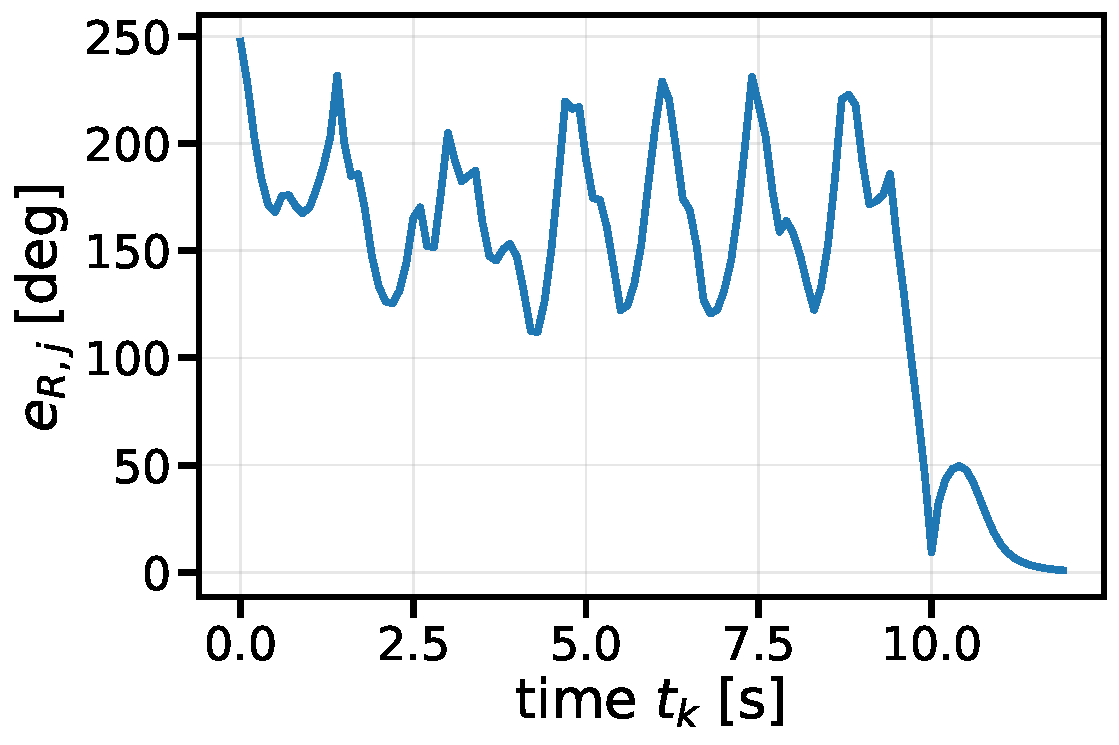
\includegraphics[width=\textwidth]{pics/Optimization/Acrobot/u5_target_rotation_error_norm.pdf}
        \caption*{(a) Target-attitude error $e_{R,j}$.}
    \end{minipage}
    \hfill
    \begin{minipage}{0.49\textwidth}
        \centering
        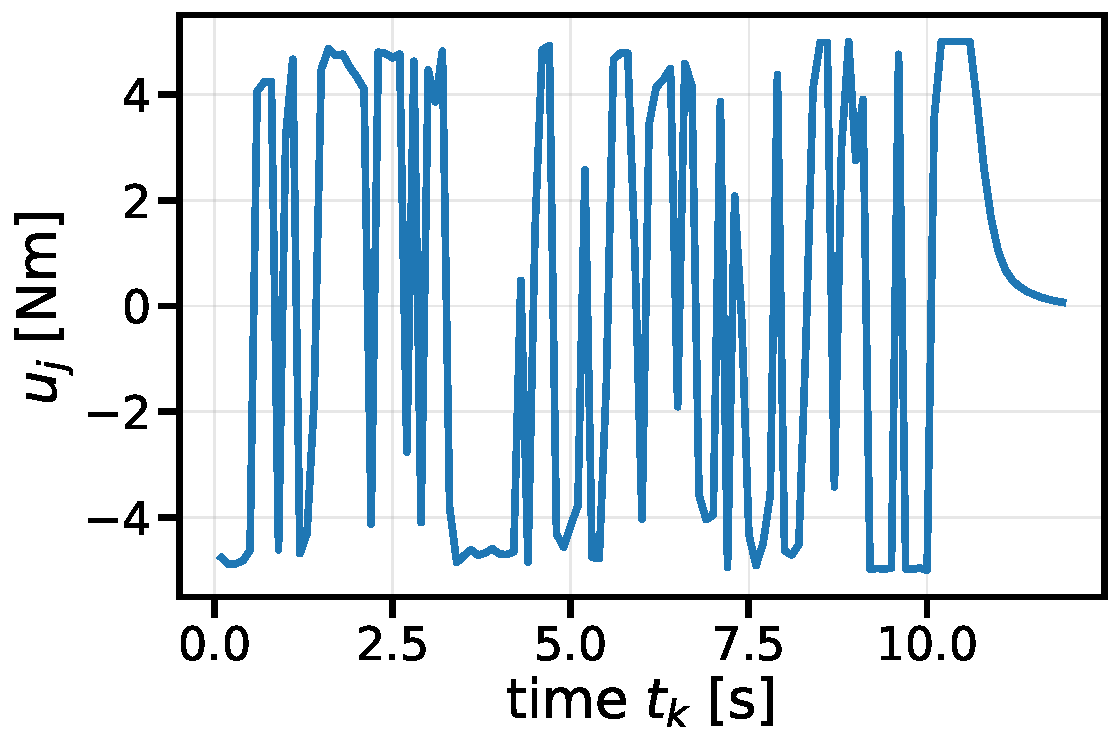
\includegraphics[width=\textwidth]{pics/Optimization/Acrobot/u5_control_inputs.pdf}
        \caption*{(b) Applied MPC control input $u_j$.}
    \end{minipage}

    \vspace{0.5em}

    \begin{minipage}{0.49\textwidth}
        \centering
        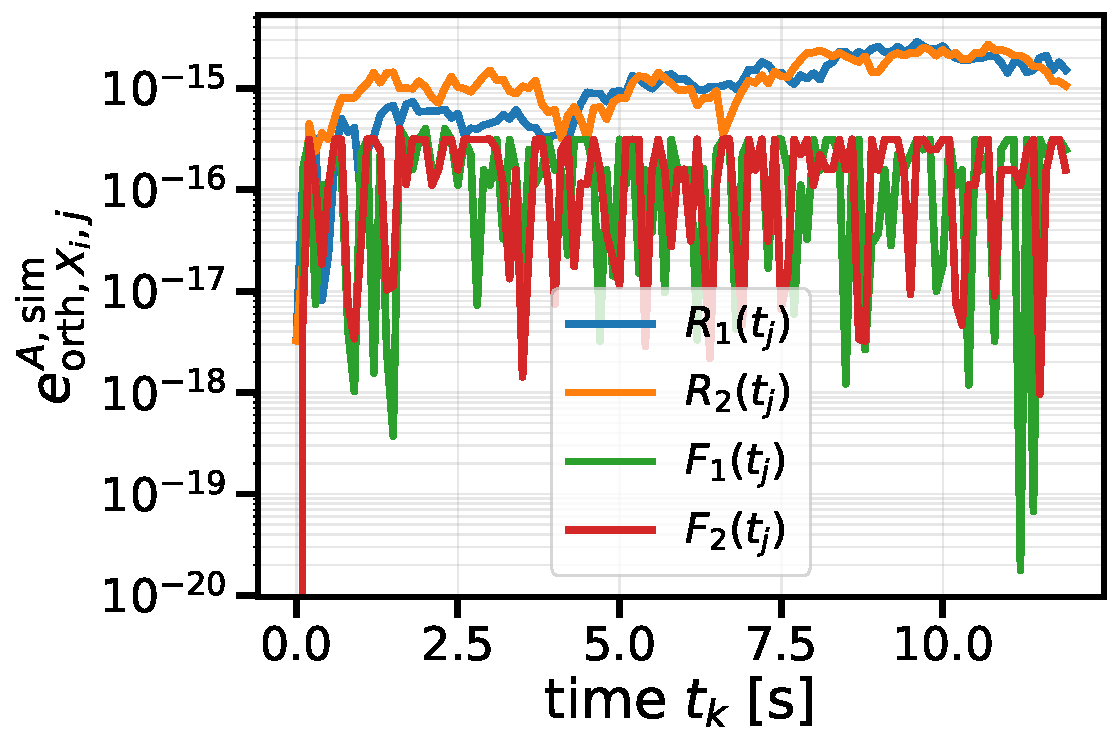
\includegraphics[width=\textwidth]{pics/Optimization/Acrobot/u5_SO2_errors_R_F.pdf}
        \caption*{(c) $SO(2)$ errors of $\bm{X}_{i,j}$.}
    \end{minipage}
    \hfill
    \begin{minipage}{0.49\textwidth}
        \centering
        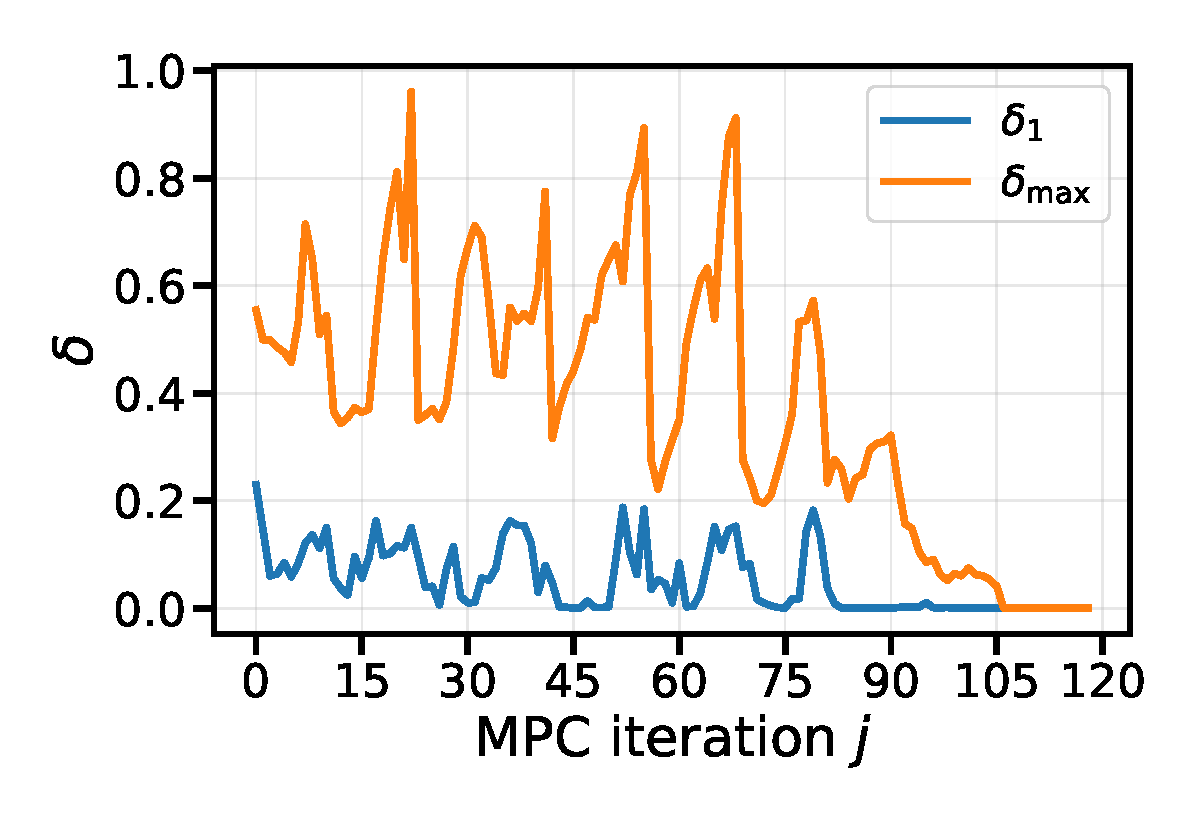
\includegraphics[width=\textwidth]{pics/Optimization/Acrobot/rank_condition_u5.pdf}
        \caption*{(d) Rank metrics $\delta_1$ and $\delta_{\max}$.}
    \end{minipage}

    \caption{Closed-loop SDP--MPC results for the Acrobot with
    $u_{\max}=5\,\mathrm{N\,m}$.}
    \label{fig:acrobot_mpc_u5_closed_loop}
\end{figure}

\paragraph{Results for $u_{\max}=5\,\mathrm{N\,m}$}
Figure \ref{fig:acrobot_mpc_u5_closed_loop} shows one successful closed-loop
swing-up and achieved stabilization. The combined starting attitude error
$e_{R,1}^A$ at $j=1$ is approximately
$247.5^\circ$. The error remains large and oscillates during
the swing up sequence. It begins to decrease rapidly after
approximately $9.5\,\mathrm{s}$ and remains close to zero after approximately
$11.9\,\mathrm{s}$. Therefore, the controller generates a swing-up motion
before stabilizing the Acrobot near the inverted equilibrium (see Fig \ref{fig:acrobot_mpc_u5_closed_loop}(a)).

In Fig.~\ref{fig:acrobot_mpc_u5_closed_loop}(b), the control input repeatedly reaches both limits of
$\pm5\,\mathrm{N\,m}$ during most of the swing-up and decreases toward zero
near the target. The torque constraint is therefore active and restricts
the available corrective action. 

Fig.~\ref{fig:acrobot_mpc_u5_closed_loop}(c) 
illustrates that
the orthogonality errors of the simulated $\bm R_i$ and $\bm F_i$ remain
below $10^{-15}$ without a growing drift. 
Therefore, the generated numerical LGVI trajectory remains
on $SO(2)$. However, the
raw predicted trajectories extracted from the individual SDP problems are
not feasible.

The rank metrics in Fig.~\ref{fig:acrobot_mpc_u5_closed_loop}(d) gives the
corresponding relaxation diagnostic. During a large part of the experiment,
$\delta_1$ assumes values up to approximately $0.2$, while
$\delta_{\max}$ reaches values close to $1$. The first moment block is
therefore generally closer to rank one than the worst block over the horizon.
Still it is not rank one throughout the full
swing-up process. The two metrics are simultaneously close to zero only near
stabilization. 

Finally, the implemented closed-loop SDP optimization
establishes a successful numerical closed-loop
stabilization for the considered initial state. Nevertheless,
the SDP-predicted trajectories do not provide a global optimality 
certificate for the applied control sequence.

The $5\,\mathrm{N\,m}$ bound was not sufficient across all additional tested
initial configurations. For configurations that require
stronger counteracting torques, the controller has limited capability
to provide sufficient corrective action. The following evaluation 
therefore increases the bound to 
$u_{\max}=15\,\mathrm{N\,m}$ and investigates a grid of initial link
orientations.

\paragraph{Empirical basin of attraction and time-discretization mismatch}
For this evaluation, the physical parameters, the relaxation order $\kappa=2$,
the target in \eqref{eq:acrobot_stabilization_target}, the objective
parameters, the multiplier and step-angle bounds, and the special multi-body cliques remain unchanged. Of the optimization bounds, only the control
bound is increased to $u_{\max}=15\,\mathrm{N\,m}$. Three combinations 
of prediction, simulation,
and control time scales are considered, as summarized in
Table~\ref{tab:acrobot_mpc_time_scale_cases}.

\begin{table}[!htbp]
    \centering
    \caption{Time-scale configurations used for the sampled SDP--MPC
    stabilization regions with $u_{\max}=15\,\mathrm{N\,m}$.}
    \label{tab:acrobot_mpc_time_scale_cases}
    \setlength{\tabcolsep}{7pt}
    \renewcommand{\arraystretch}{1.15}
    \begin{tabular}{@{}cccccc@{}}
        \toprule
        Case & $\Delta t_{\mathrm{SDP}}$ & $\Delta t_{\mathrm{sim}}$
        & $\Delta t_{\mathrm{ctrl}}$ & $N_{\mathrm{SDP}}$ & Time scales \\
        \midrule
        I   & $0.1\,\mathrm{s}$  & $0.1\,\mathrm{s}$
            & $0.1\,\mathrm{s}$   & $20$ & matched \\
        II  & $0.05\,\mathrm{s}$ & $0.05\,\mathrm{s}$
            & $0.05\,\mathrm{s}$  & $40$ & matched \\
        III & $0.1\,\mathrm{s}$  & $0.0025\,\mathrm{s}$
            & $0.025\,\mathrm{s}$ & $20$ & mismatched \\
        \bottomrule
    \end{tabular}
\end{table}

In both Cases~I and II, the prediction, plant, and control intervals are
matched. In both cases, the total prediction horizon is
$N_{\mathrm{SDP}}\Delta t_{\mathrm{SDP}}=2.0\,\mathrm{s}$. Case II
therefore evaluates whether a consistent refinement of all time scales changes
the sampled stabilization result while retaining approximately the same
prediction horizon time. In Case III, the prediction model uses the same
$0.1\,\mathrm{s}$ step as Case I, but the simulation model uses
fine LGVI steps of $\Delta t_{\mathrm{sim}}=0.0025\,\mathrm{s}$ 
and simulates for $\Delta t_{\mathrm{ctrl}}=0.025\,\mathrm{s}$, which corresponds to
$10$ LGVI steps per control interval. Therefore, Case~III introduces 
a temporal-discretization mismatch between
the SDP prediction and its fine closed-loop execution.

For each case, both links start at rest and their initial absolute orientations
are selected from
\begin{equation}
    \theta_1^{\mathrm{init}},\theta_2^{\mathrm{init}}
    \in\{0^\circ,20^\circ,\ldots,180^\circ\}.
\label{eq:acrobot_mpc_basin_initial_grid}
\end{equation}
All $10\times10=100$ combinations are evaluated directly. 
The same stabilization tolerances $\varepsilon_R=2^\circ$ and
$\varepsilon_F=2^\circ$ are used in all cases.
\begin{figure}[!t]
    \centering
    \captionsetup{skip=0pt}
    \begin{minipage}[t]{0.45\textwidth}
        \centering
        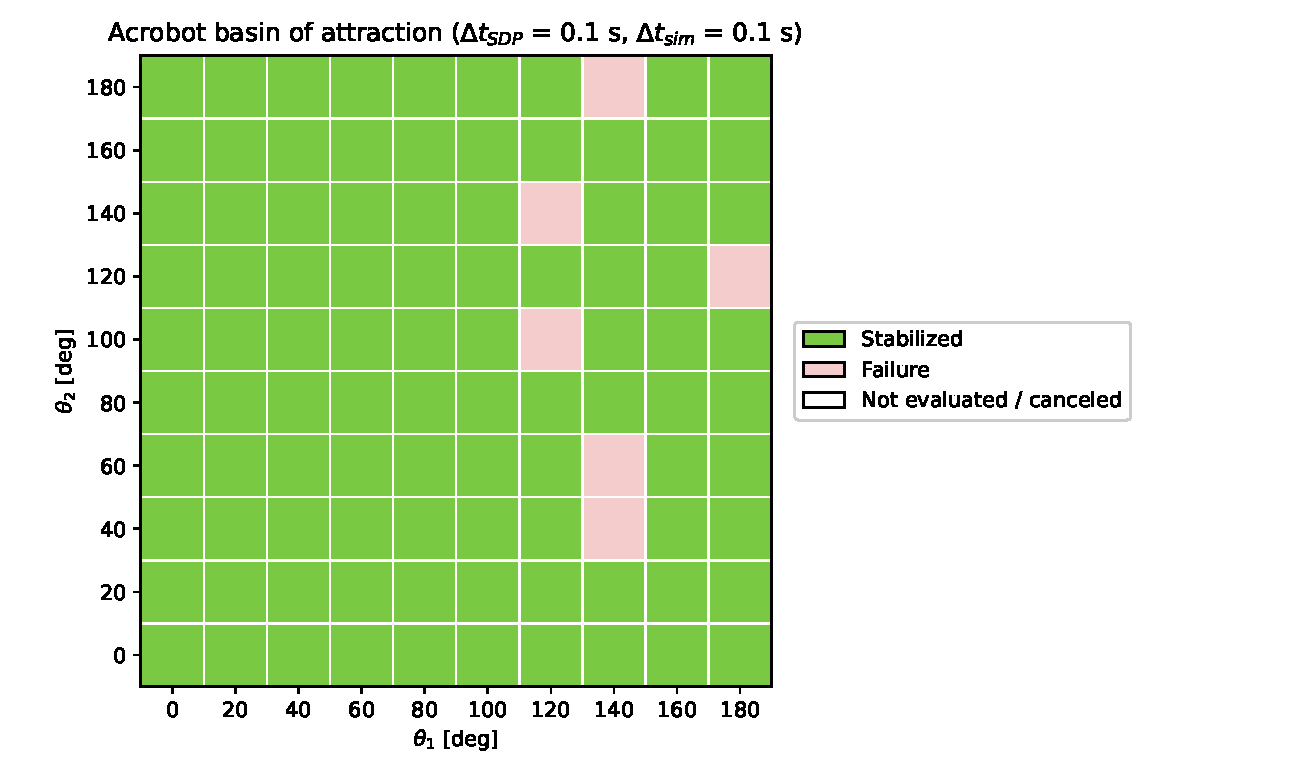
\includegraphics[width=\textwidth,trim=0 1.9cm 0 0,clip]{pics/Optimization/Acrobot/basin_of_attraction_01.pdf}
        \caption*{(a) Case~I.}
    \end{minipage}
    \hfill
    \begin{minipage}[t]{0.45\textwidth}
        \centering
        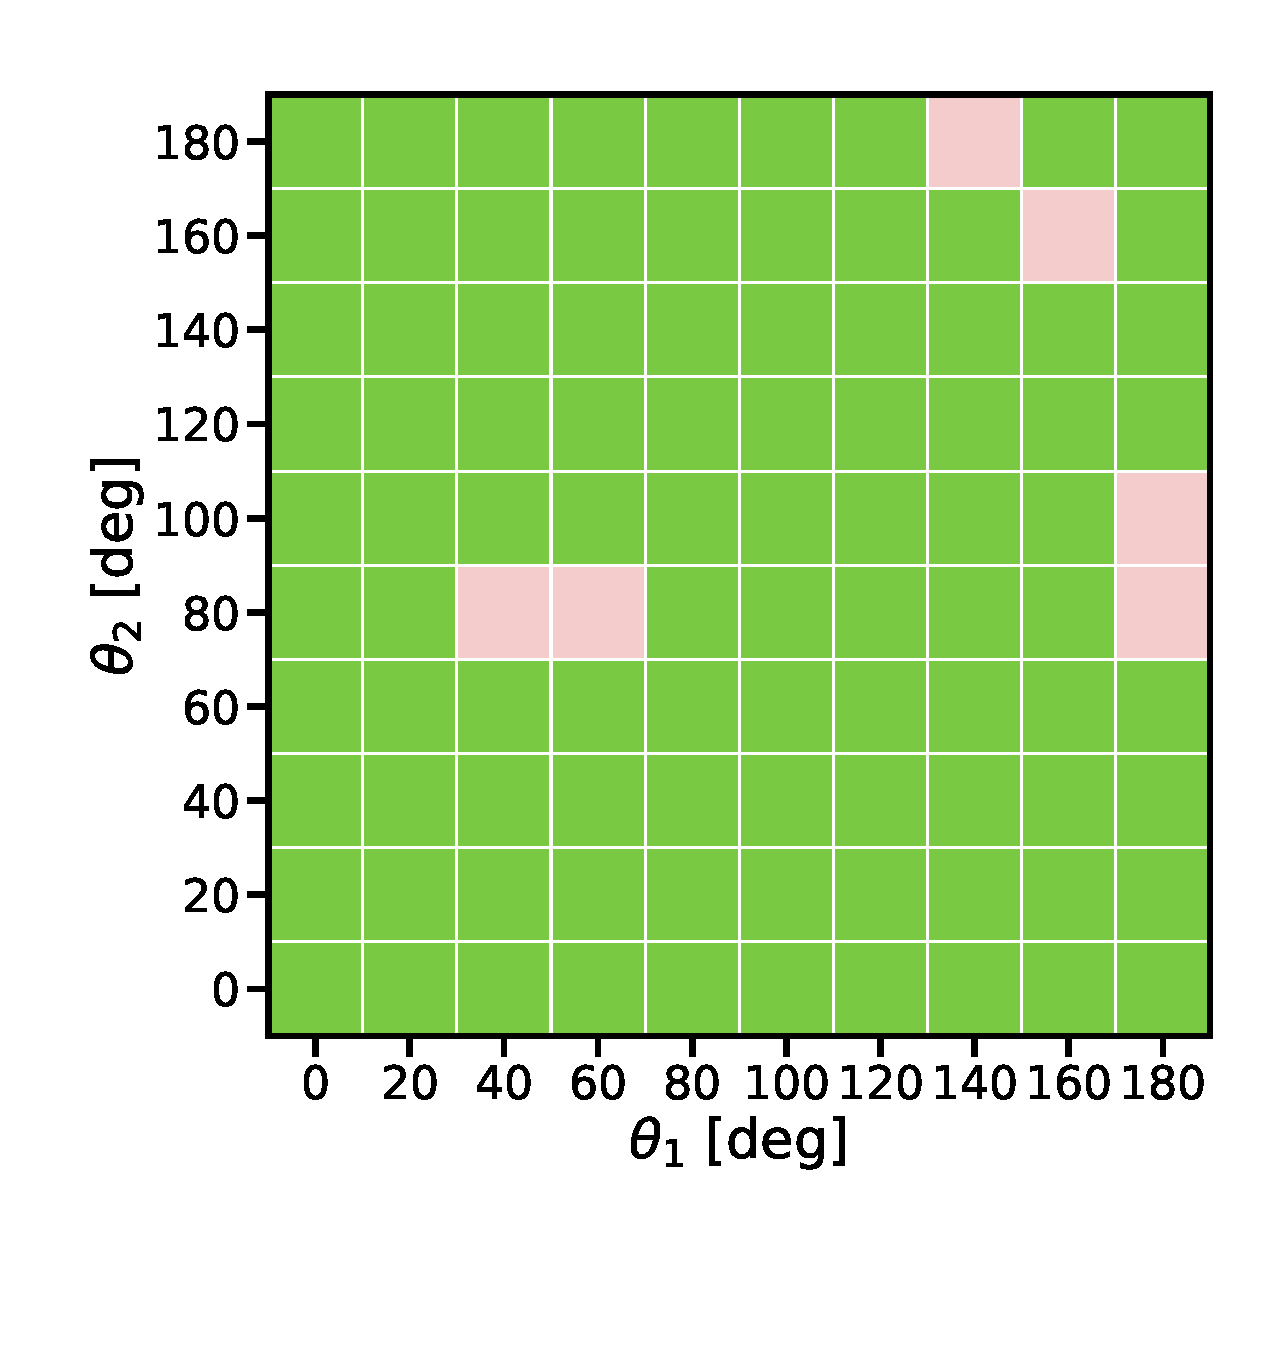
\includegraphics[width=\textwidth,trim=0 1.9cm 0 0,clip]{pics/Optimization/Acrobot/basin_of_attraction_005.pdf}
        \caption*{(b) Case~II.}
    \end{minipage}
    \par\medskip
    \begin{minipage}[t]{0.45\textwidth}
        \centering
        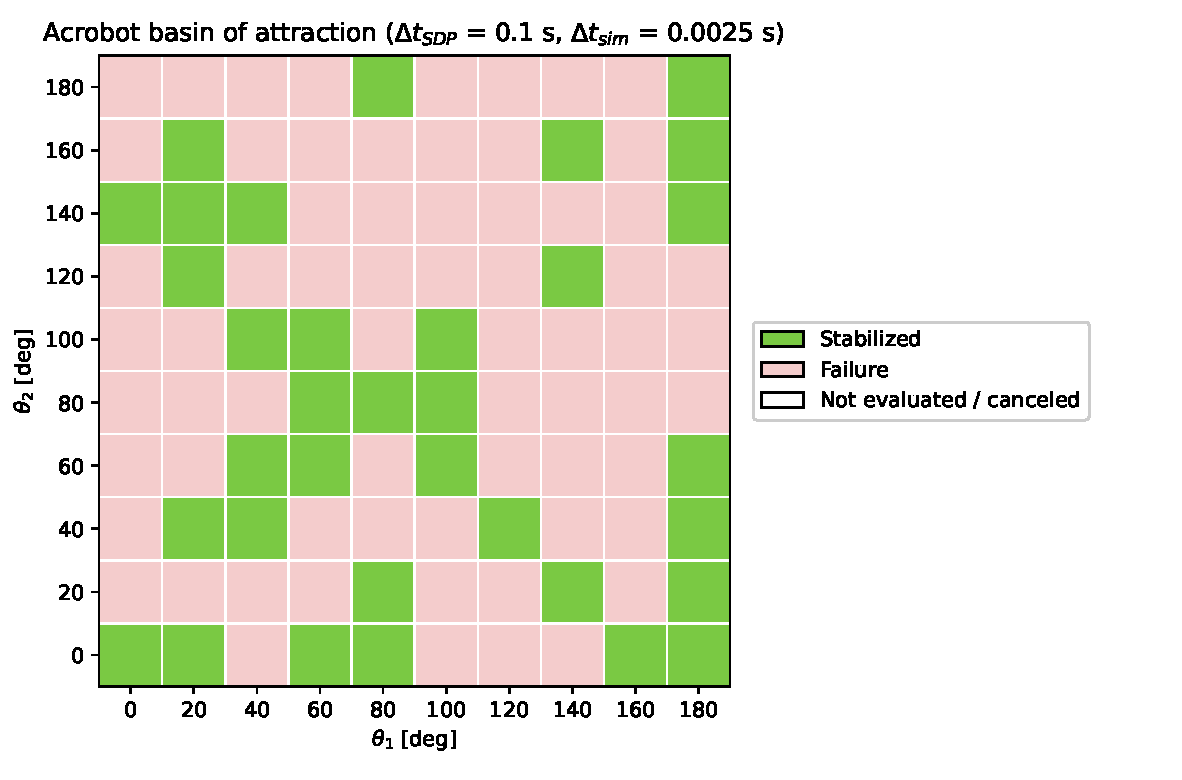
\includegraphics[width=\textwidth,trim=0 1.9cm 0 0,clip]{pics/Optimization/Acrobot/basin_of_attraction_00025.pdf}
        \caption*{(c) Case~III.}
    \end{minipage}

    \vspace{0.9\baselineskip}
    \caption{Empirical sampled stabilization regions of the SDP-MPC
    controller with $u_{\max}=15\,\mathrm{N\,m}$. The tuples
    $(\Delta t_{\mathrm{SDP}},\Delta t_{\mathrm{sim}},
    \Delta t_{\mathrm{ctrl}})$ are $(0.1,0.1,0.1)\,\mathrm{s}$ in Case~I,
    $(0.05,0.05,0.05)\,\mathrm{s}$ in Case~II, and
    $(0.1,0.0025,0.025)\,\mathrm{s}$ in Case~III.}
    \label{fig:acrobot_basin_comparison}
\end{figure}

Figures~\ref{fig:acrobot_basin_comparison} (a)-(b) show that the Acrobot 
model stabilizes $94$ of the $100$ 
initial configurations in Case~I. The matched time-scale configuration
of Case II also contains $94$ stabilized samples, although the locations
of the six non-stabilized entries changed. Therefore, reducing all three time steps
from $0.1\,\mathrm{s}$ to $0.05\,\mathrm{s}$ does not change the overall
stabilization success. Here, the failures occur
after the SDP optimization returns an infeasible solution. 

In contrast, only $34$ of the $100$ samples are marked as stabilized in
Case III, illustrated in Figure~\ref{fig:acrobot_basin_comparison} (c). 
The successful samples form a scattered set rather than a contiguous
region and occur primarily for easier configurations for 
$\theta_1 < 100^\circ$ or configurations 
in which link $i=1$ is already relatively close to the $180^\circ$ target. 
However, both groups are interrupted by failures. Moreover, only five of the thirty samples in the region
$120^\circ\leq\theta_1\leq160^\circ$ stabilize.
The increase in failure states cannot be explained only
by the smaller $\Delta t_{sim}$, as Case~II also refines
the prediction, simulation, and control intervals consistently, but without reducing
the total number of stabilized samples. Instead, the comparison between 
Case~I-II and Case~III indicates that 
the mismatched time scales in Case~III lead to increased failure rates. 
However, a possible case with 
$\Delta t_{SDP}=\Delta t_{sim}=\Delta t_{ctrl}=0.0025\,\mathrm{s}$
could not be evaluated due to the high computational cost of solving the SDP
problems with $N_{\mathrm{SDP}}=800$.

For the successfully stabilized initial configuration
$\theta_{1,\mathrm{init}}=\theta_{2,\mathrm{init}}=80^\circ$, the complete SDP-MPC 
computation required approximately $3.1\,\mathrm{h}$ in Case~I, $27.3\,\mathrm{h}$ in Case~II, 
and $17.8\,\mathrm{h}$ in Case~III. The runtime is determined first by $\Delta t_{\mathrm{SDP}}$ and 
$N_{\mathrm{SDP}}$, which define the size and cost of each SDP problem, and second by the time-discretization mismatch, 
which can increase the number of MPC iterations required before stabilization.

\begin{figure}[!t]
    \centering
    \begin{minipage}[t]{0.49\textwidth}
        \centering
        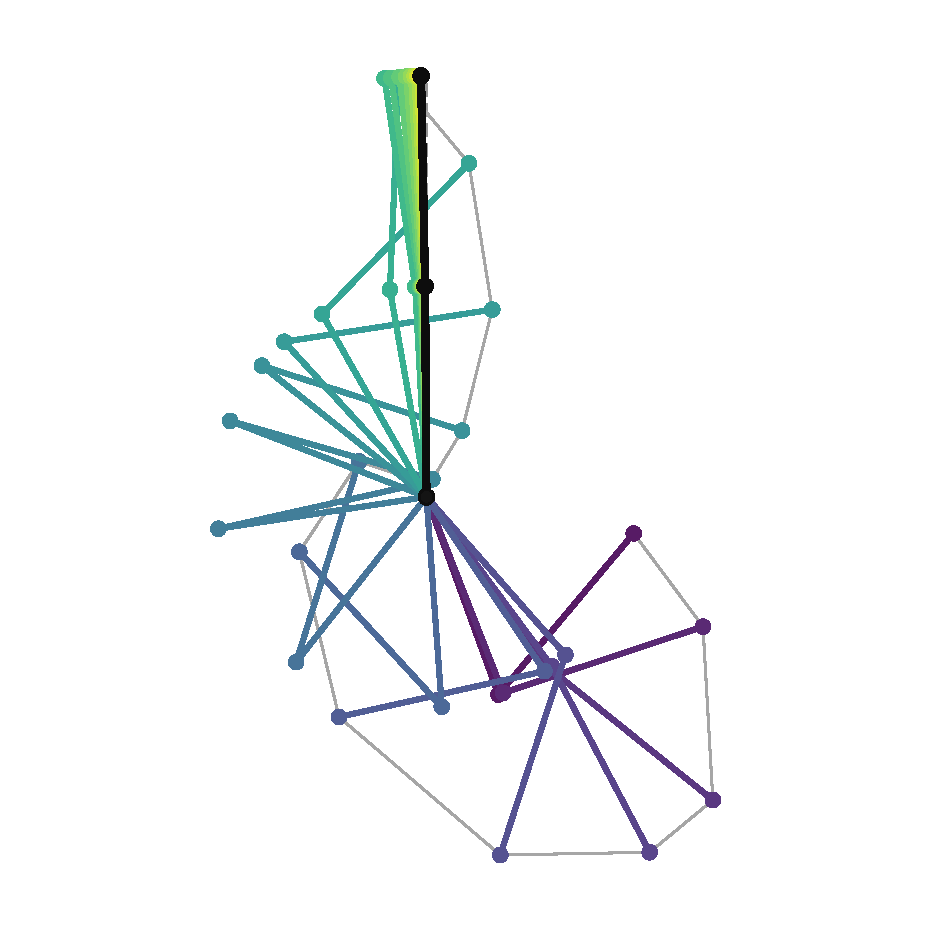
\includegraphics[width=\textwidth]{pics/Optimization/Acrobot/acrobot_trajectory_01_01_01.pdf}
        \caption*{(a) Case~I: $(0.1,0.1,0.1)\,\mathrm{s}$.}
    \end{minipage}
    \hfill
    \begin{minipage}[t]{0.49\textwidth}
        \centering
        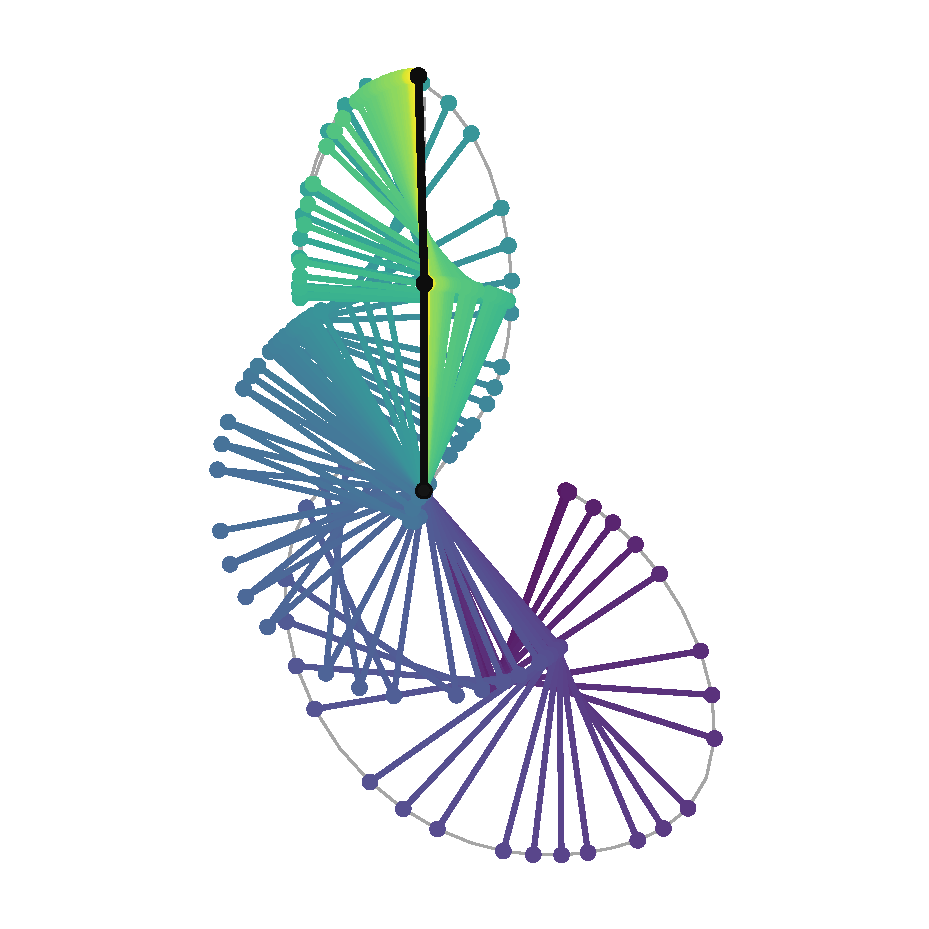
\includegraphics[width=\textwidth]{pics/Optimization/Acrobot/acrobot_trajectory_01_00025_0025.pdf}
        \caption*{(b) Case~III: $(0.1,0.0025,0.025)\,\mathrm{s}$.}
    \end{minipage}

    \caption{Closed-loop Acrobot tip trajectories and sampled link
    configurations for
    $(\theta_1^{\mathrm{init}},\theta_2^{\mathrm{init}})
    =(20^\circ,140^\circ)$ in Cases~I and III. Each tuple gives
    $(\Delta t_{\mathrm{SDP}},\Delta t_{\mathrm{sim}},
    \Delta t_{\mathrm{ctrl}})$.}
    \label{fig:acrobot_sampled_trajectory_comparison}
\end{figure}

The trajectory comparison in
Fig.~\ref{fig:acrobot_sampled_trajectory_comparison} illustrates the described
behaviour for the common initial configuration
$(\theta_1^{\mathrm{init}},\theta_2^{\mathrm{init}})
=(20^\circ,140^\circ)$. With matched $0.1\,\mathrm{s}$ time scales, the
Acrobot follows a comparatively direct swing-up and satisfies the stabilization
criterion after approximately $2.2\,\mathrm{s}$. The mismatched Case~III also
reaches the inverted equilibrium, but requires approximately $4.1\,\mathrm{s}$.
Its link-tip paths contain considerably larger loops, and the repeated passages
around the upright configuration indicate a more oscillatory transient. Thus,
receding-horizon feedback can compensate for the temporal mismatch in this
particular case, but only at the cost of a slower and less direct
closed-loop maneuver.

\paragraph{Summary}
For the evaluated initial states, the SDP-MPC controller can convert first-step
extractions into on-manifold simulated swing-ups, although the complete-horizon
moment relaxations are not generally numerically rank one. With
$u_{\max}=5\,\mathrm{N\,m}$, stabilization is obtained for the symmetric
$5^\circ$ initial state, but the limited control and unsuccessful additional
trials reveal limited control authority. Increasing the bound to
$15\,\mathrm{N\,m}$ yields broad sampled stabilization regions for matched
prediction and execution time scales, whereas the mismatched configuration
stabilizes only about one third of the tested initial states.
Although the SDP relaxations do not provide a certificate of global optimality, 
the results show that embedding the SDP optimization in a closed loop with numerical 
simulation can generate feasible stabilizing trajectories.




%\section{Experimental Results}

%A thesis almost always has an experimental part, typically some comparison to other approaches. Benchmarking takes time, for running the experiments, but also for thinking them up in the first place, and for analysing the results. Plan accordingly to spend enough time here!

%Think about what makes sense to measure, what you want to learn from your measurements. Think about what is really the relevant contribution of your thesis, and how you can prove that you have achieved your goals. Think about what you can measure in order to get a good insight into the performance of various aspects of your design, how you can distinguish between systematic and accidental effects, how you can convince yourself that your results are right. If you get surprising results, do not just say ``surprise, surprise, performance isn't as good as hoped''. Find out why. Surprises without explanation indicate either that you are clueless about what is going on, or that you have made a mistake. Unconvincing results, therefore, tend to imply unconvincing marks. 

%\paragraph{Statistics:} Measurements always have statistical (sampling) errors. Owing to the deterministic nature of simulations these are sometimes very small, as disturbing factors can be designed. However, the reader should be given an indication of how statistically significant the results are. This is done by providing at least a standard deviation in addition to averages. Whenever the results of several runs are averaged, a standard deviation can (and must) be supplied. After all, you average to reduce statistical errors.

%The reproducibility argument applies here just as much as for the implementation. Give enough detail on what you measure, and how you measure it, so that someone who has your implementation (but not your test code) or has re-done your implementation independently, should be able to repeat your measurements and arrive at essentially the same results. In some cases, results seem outright wrong in a thesis. In those cases, not enough detail is provided to allow the supervisor/reader to pinpoint the likely source of the error. Often the cause is systematic errors resulting from an incorrect measurement technique. If it seems wrong, and the text does not convince the reader that it is not wrong, the reader will assume that it is wrong.
